\documentclass[
	fontsize=11pt,
	paper=a4,
	pagesize=auto,
	parskip=full,
	titlepage=on,
	ngerman
]{scrartcl}

\usepackage[a4paper, total={16cm, 23cm}]{geometry}
\usepackage[ngerman]{babel}
\usepackage[T1]{fontenc}
\usepackage[utf8]{inputenc}
\usepackage{lmodern}

\usepackage{amsmath}
\usepackage{amssymb}
\usepackage{siunitx}
\sisetup{locale=DE}

\usepackage[hidelinks]{hyperref}

\usepackage{float}
\usepackage[final]{graphicx}
\graphicspath{ {./media/} }
\usepackage{subcaption}

\usepackage{enumitem}

\newlength{\imagewidth}

\begin{document}
\setlength{\imagewidth}{0.5\textwidth}

\section{Material}

\begin{itemize}[noitemsep]
	\item Gehäuse
	\item 4x FTF-Kabel
	\item 22x FTM-Kabel
	\item 9x MTM-Kabel
	\item 2x T-Motor
	\item Arduino Uno
	\item H-Brücke mit 9V-Block Verbinder
	\item HC05
	\item Widerstand
	\item Jumper
\end{itemize}

\section{Zusammenbau}

% \begin{figure}[H]
% 	\centering
% 	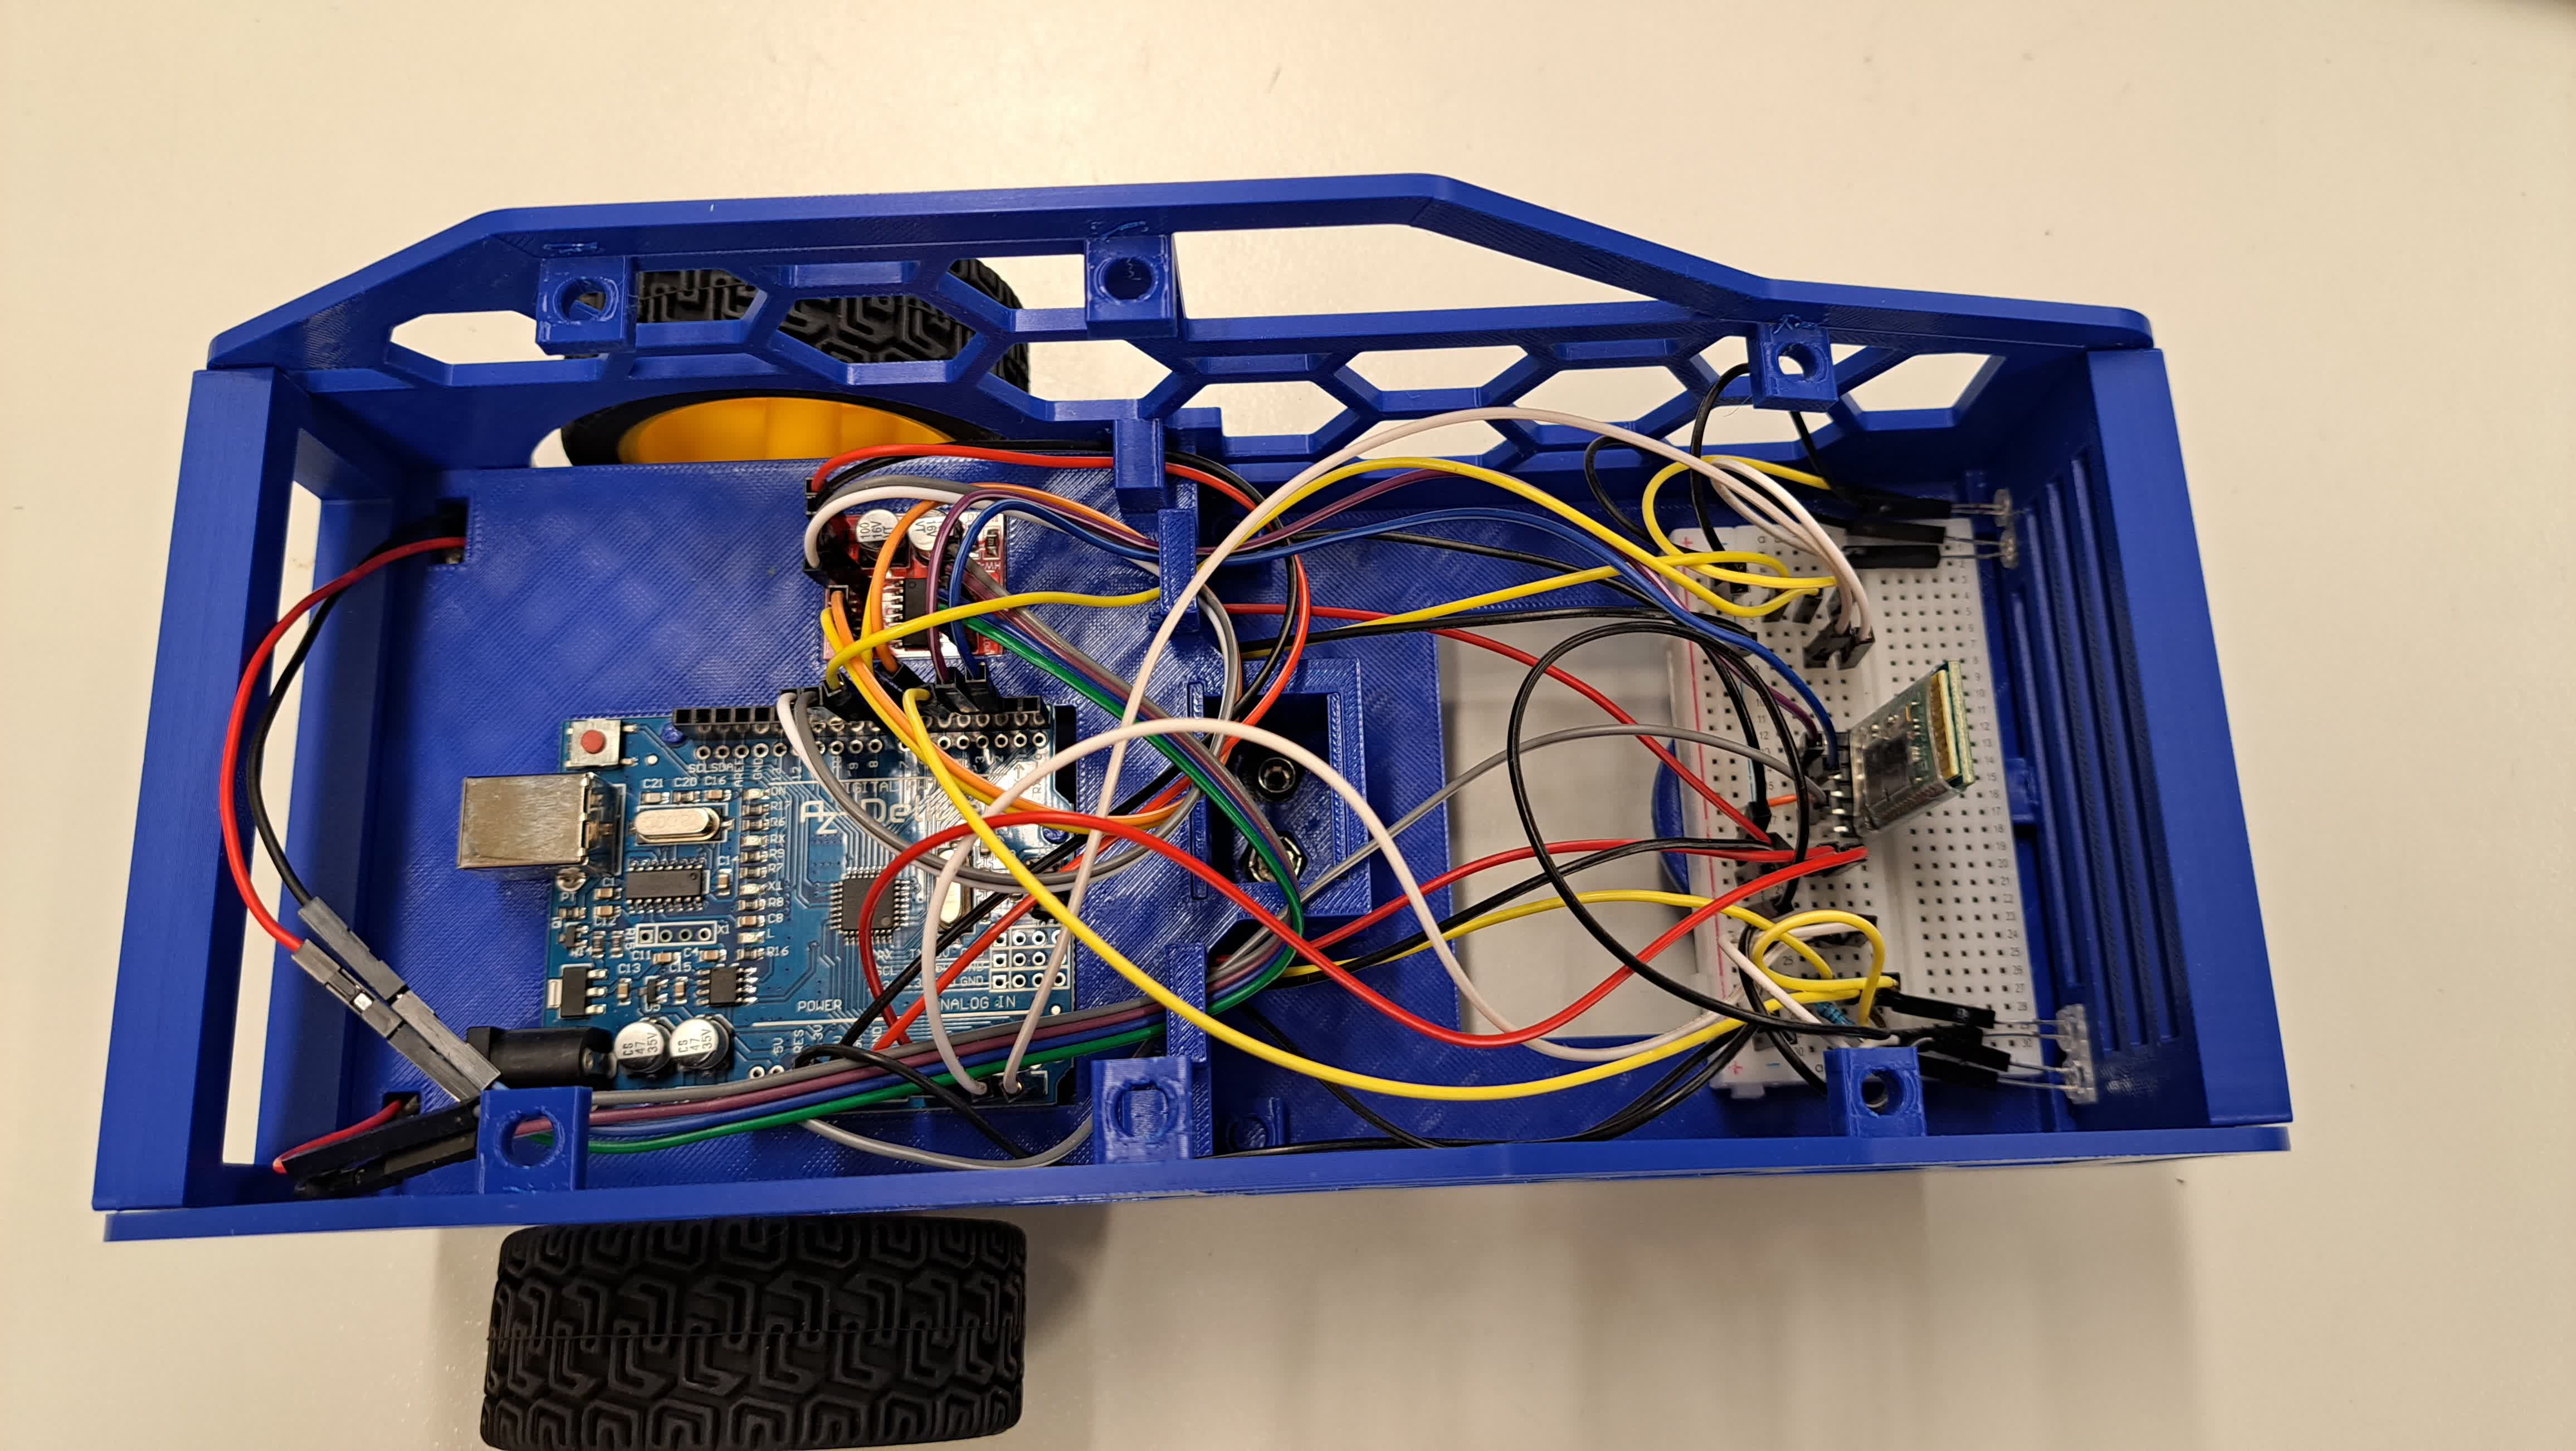
\includegraphics[width=\imagewidth]{IMG_1000}
% \end{figure}

% \begin{figure}[H]
% 	\centering
% 	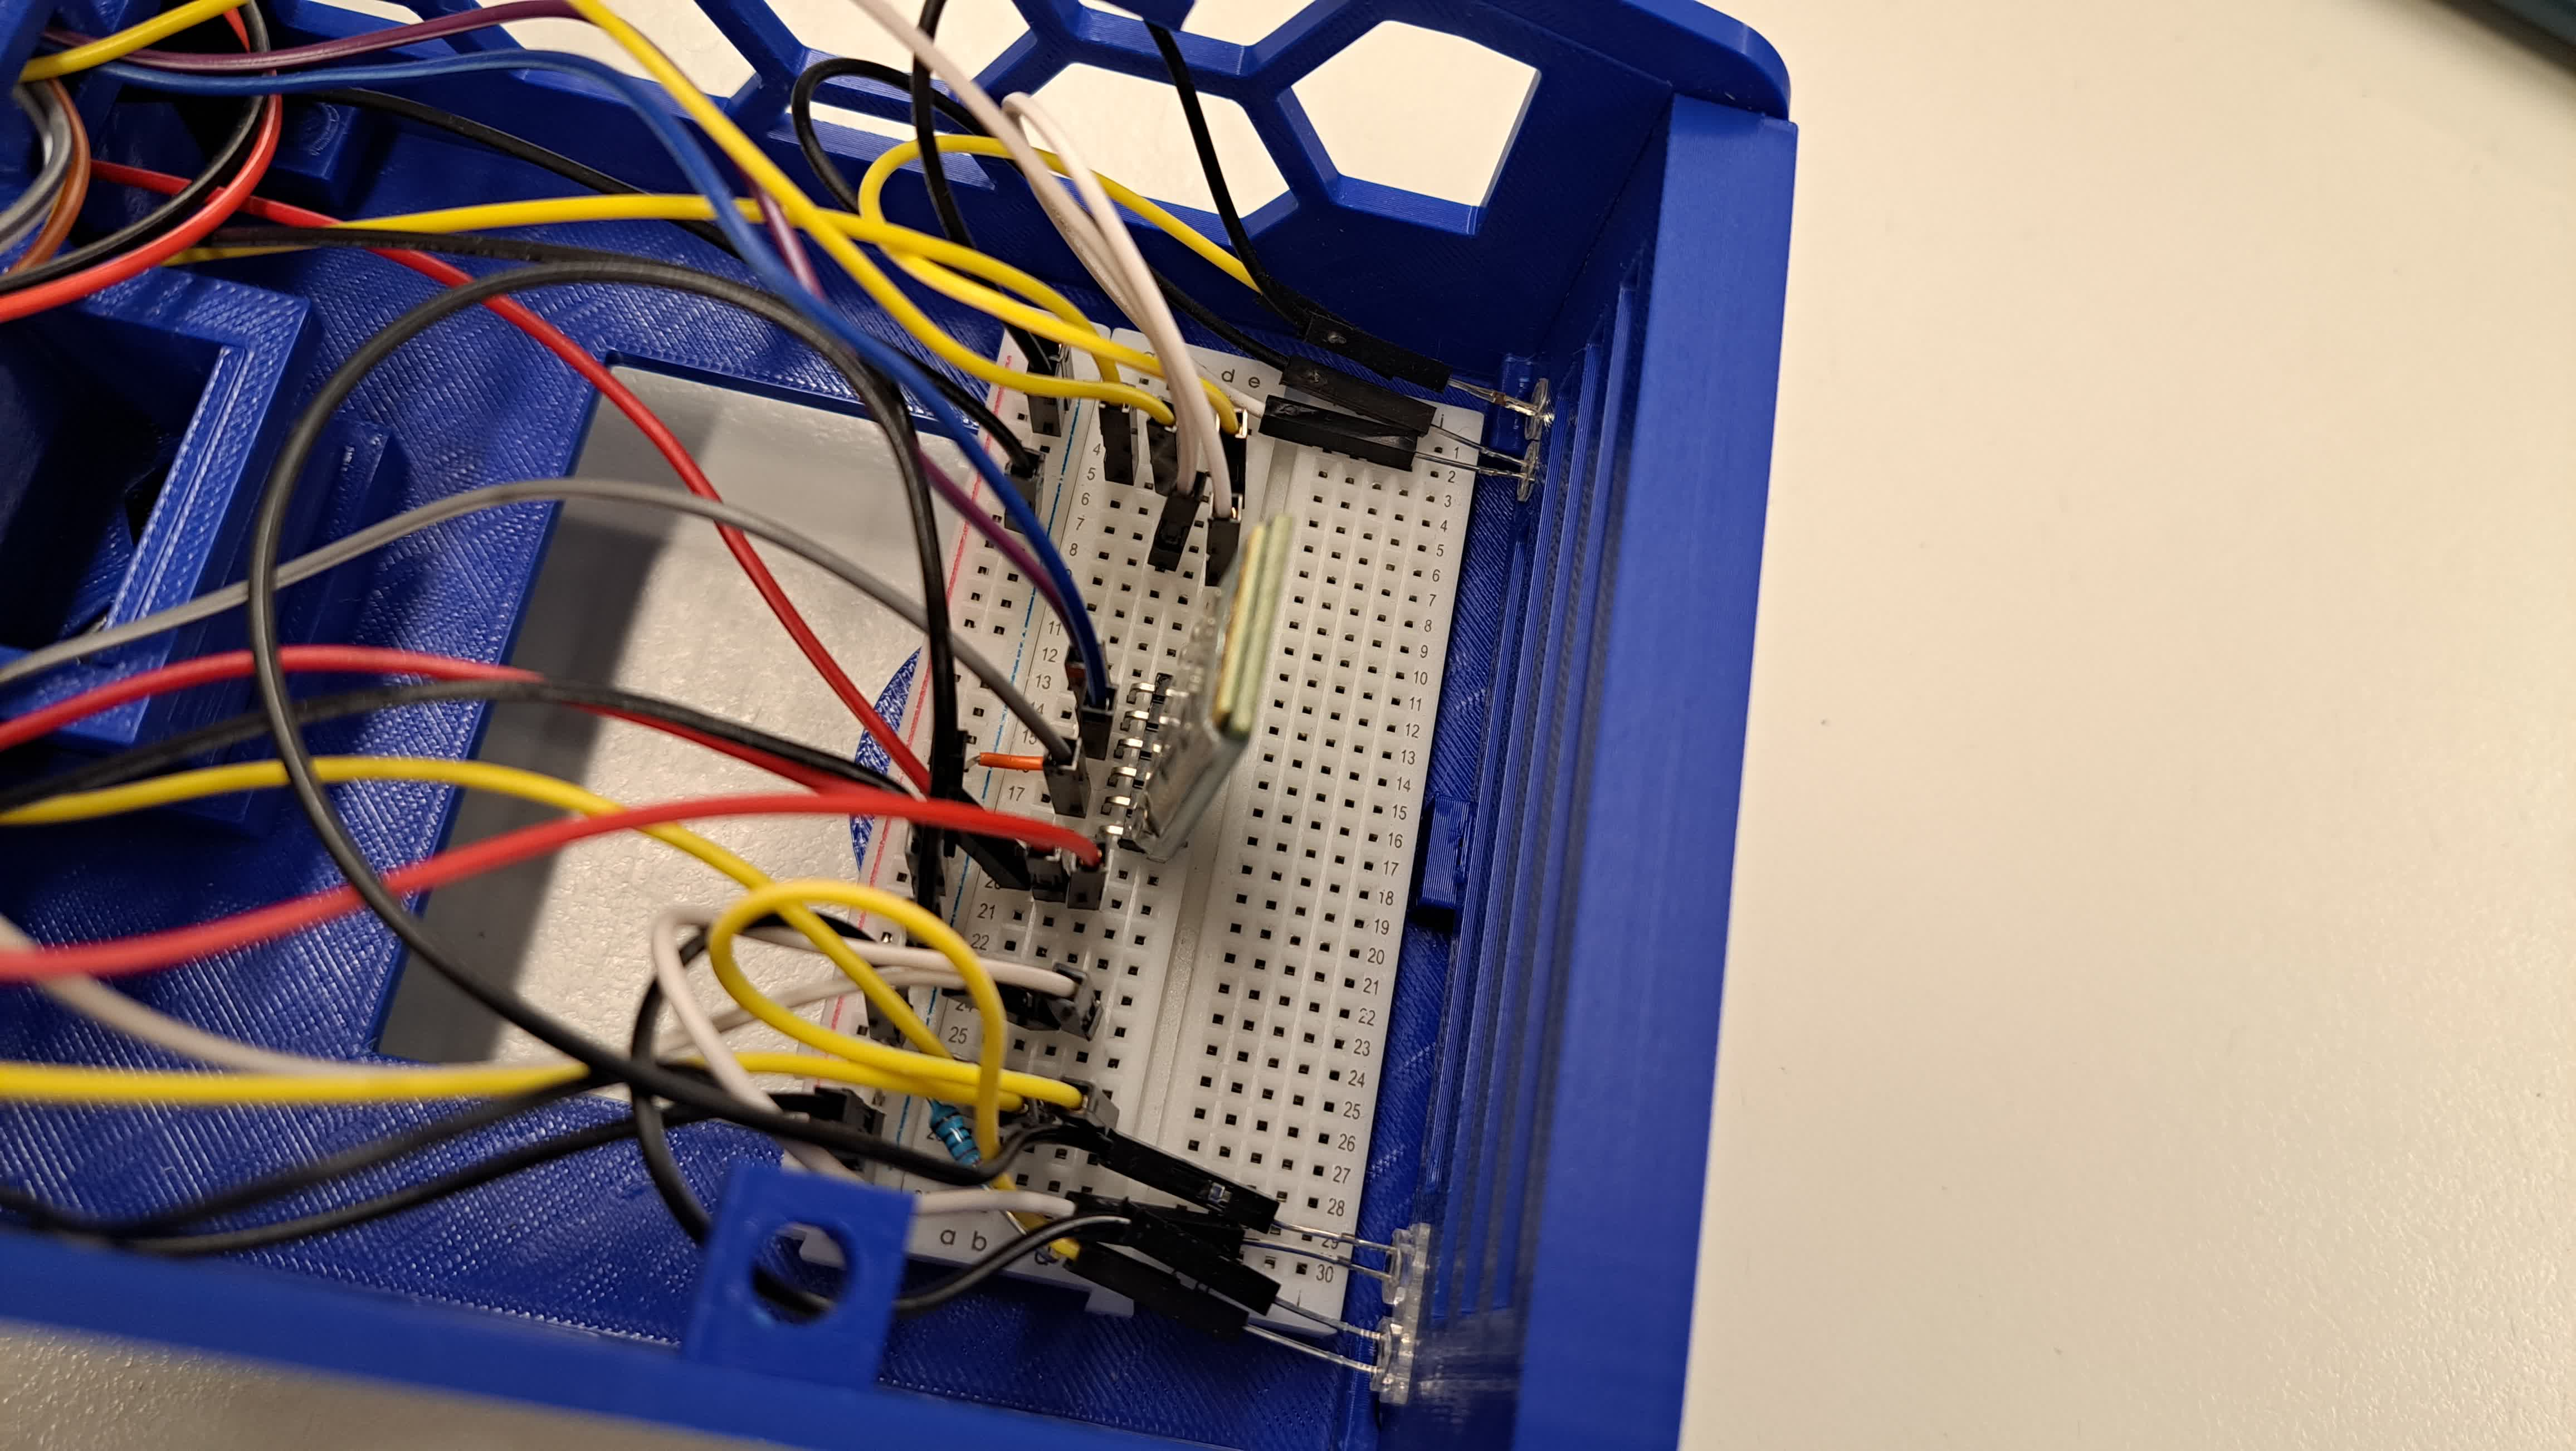
\includegraphics[width=\imagewidth]{IMG_1001}
% \end{figure}

% \begin{figure}[H]
% 	\centering
% 	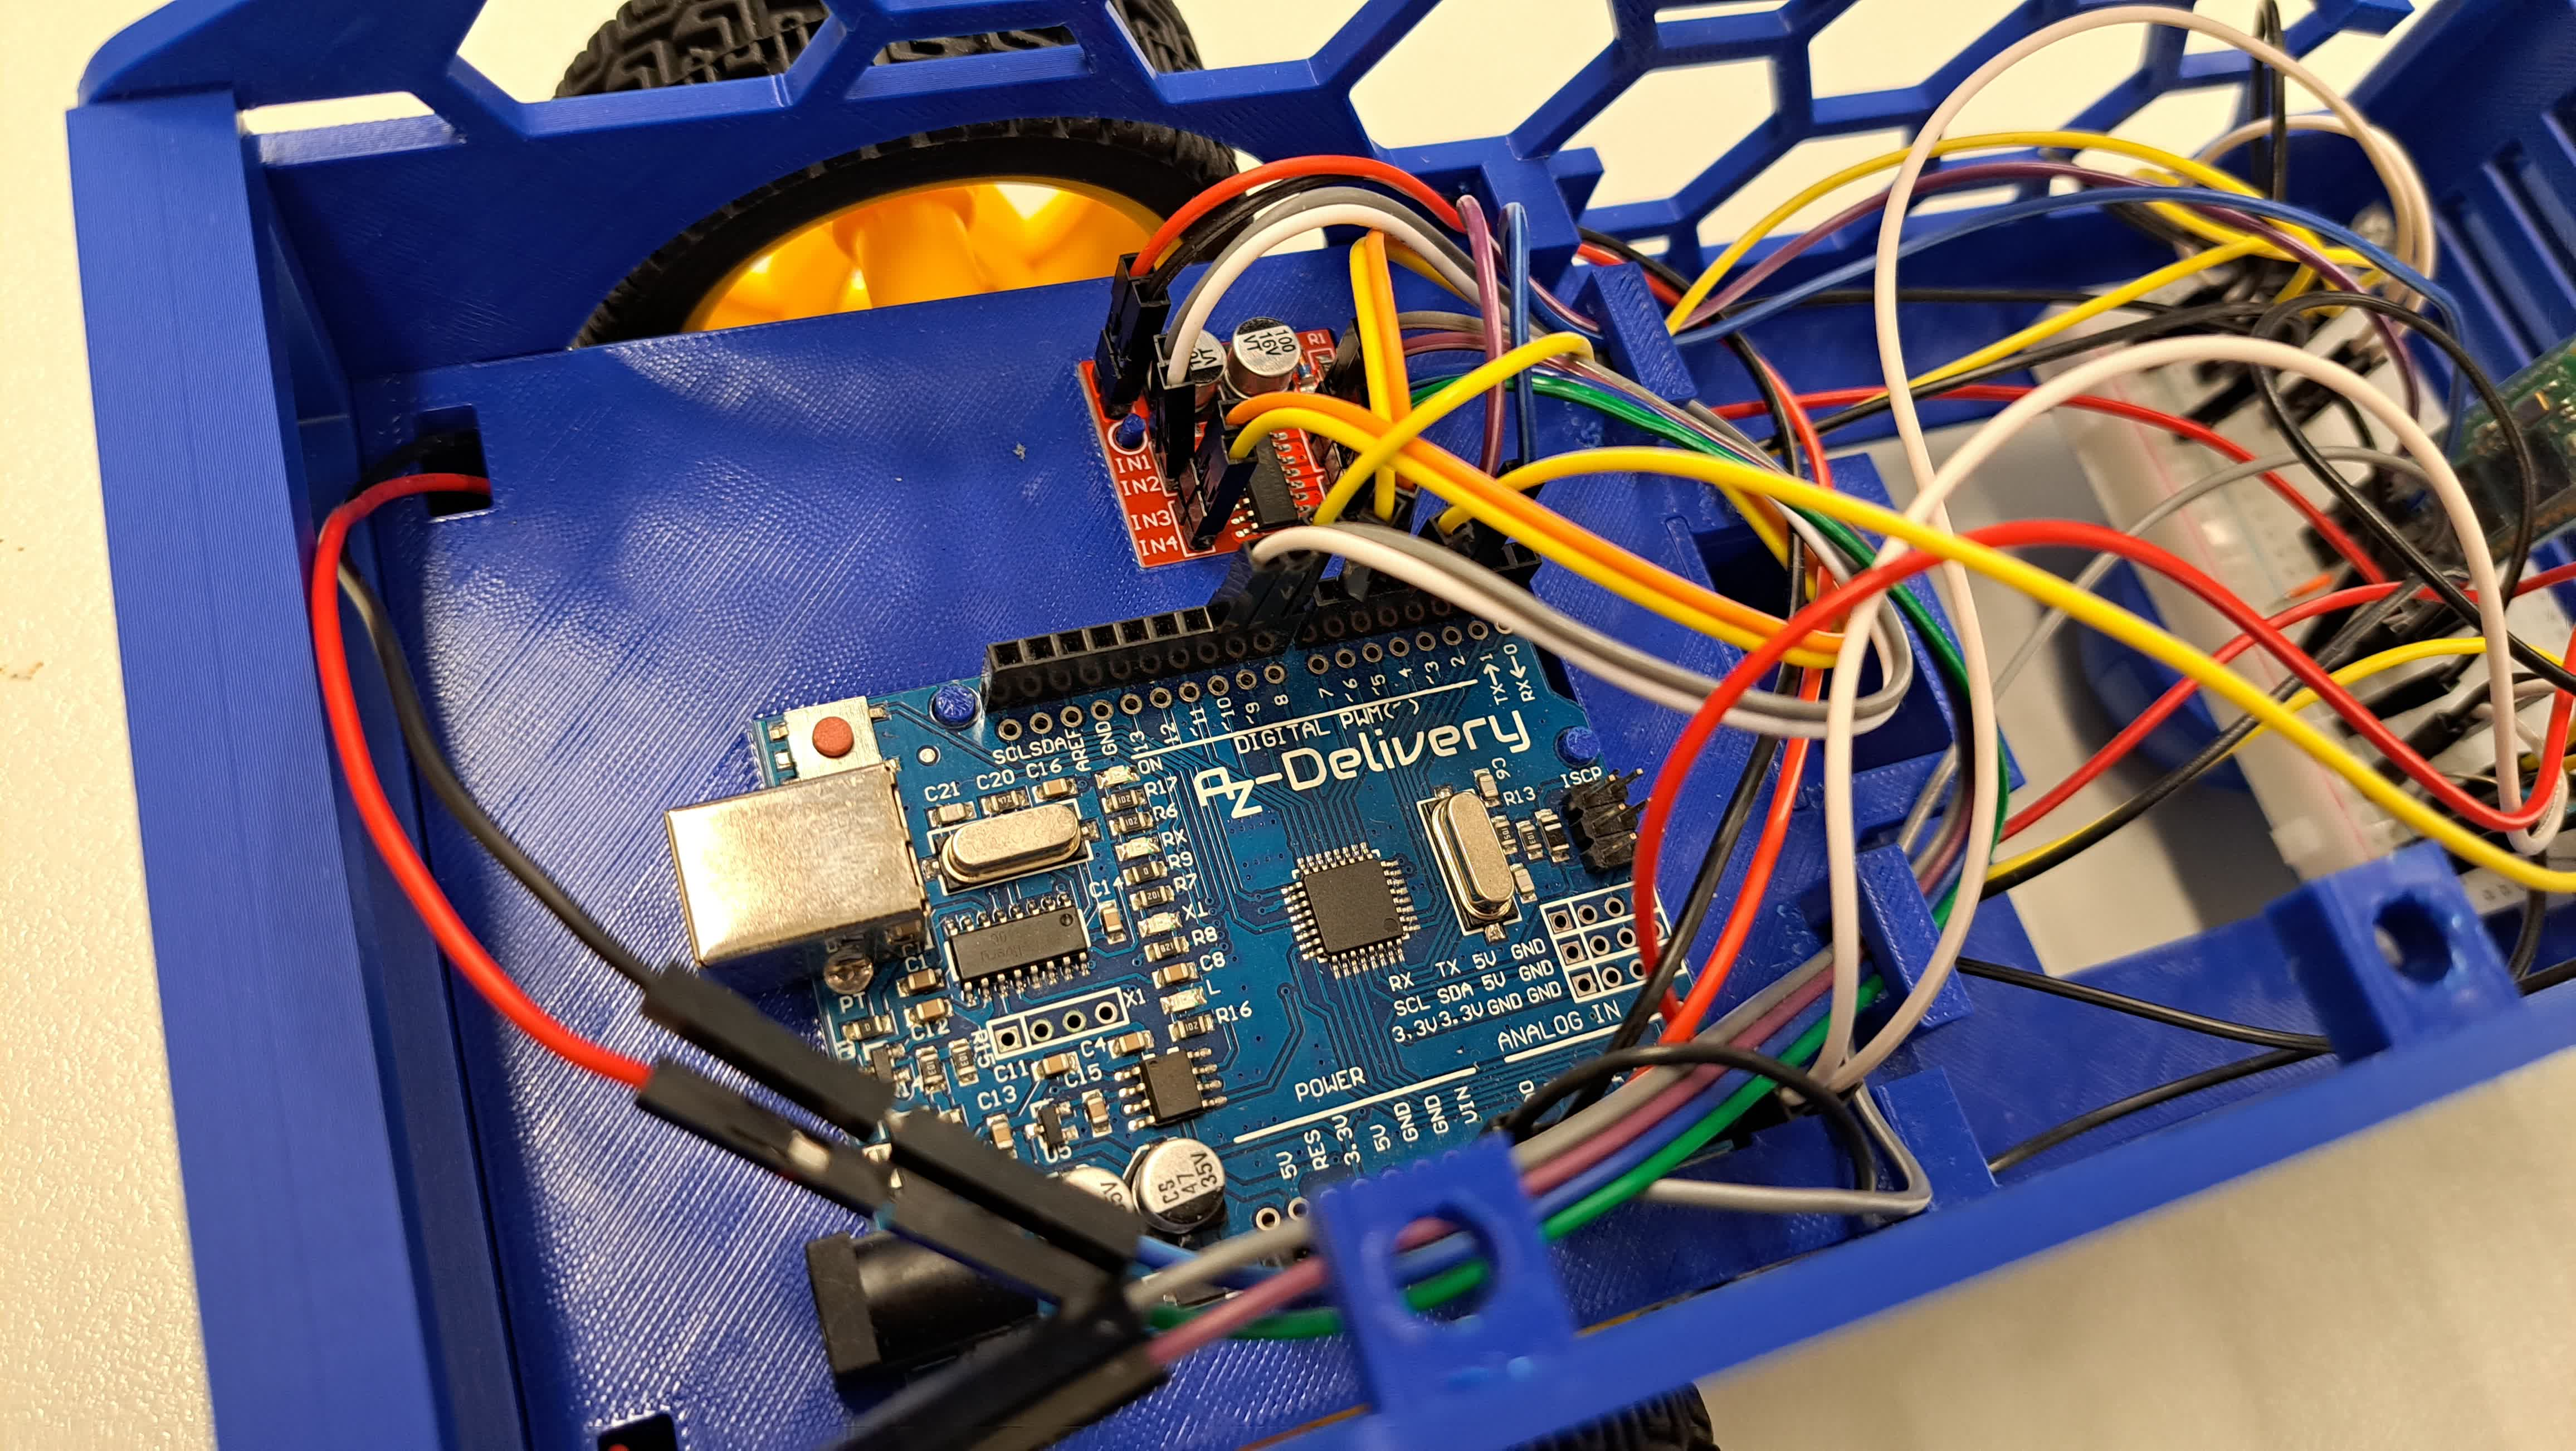
\includegraphics[width=\imagewidth]{IMG_1002}
% \end{figure}

% \begin{figure}[H]
% 	\centering
% 	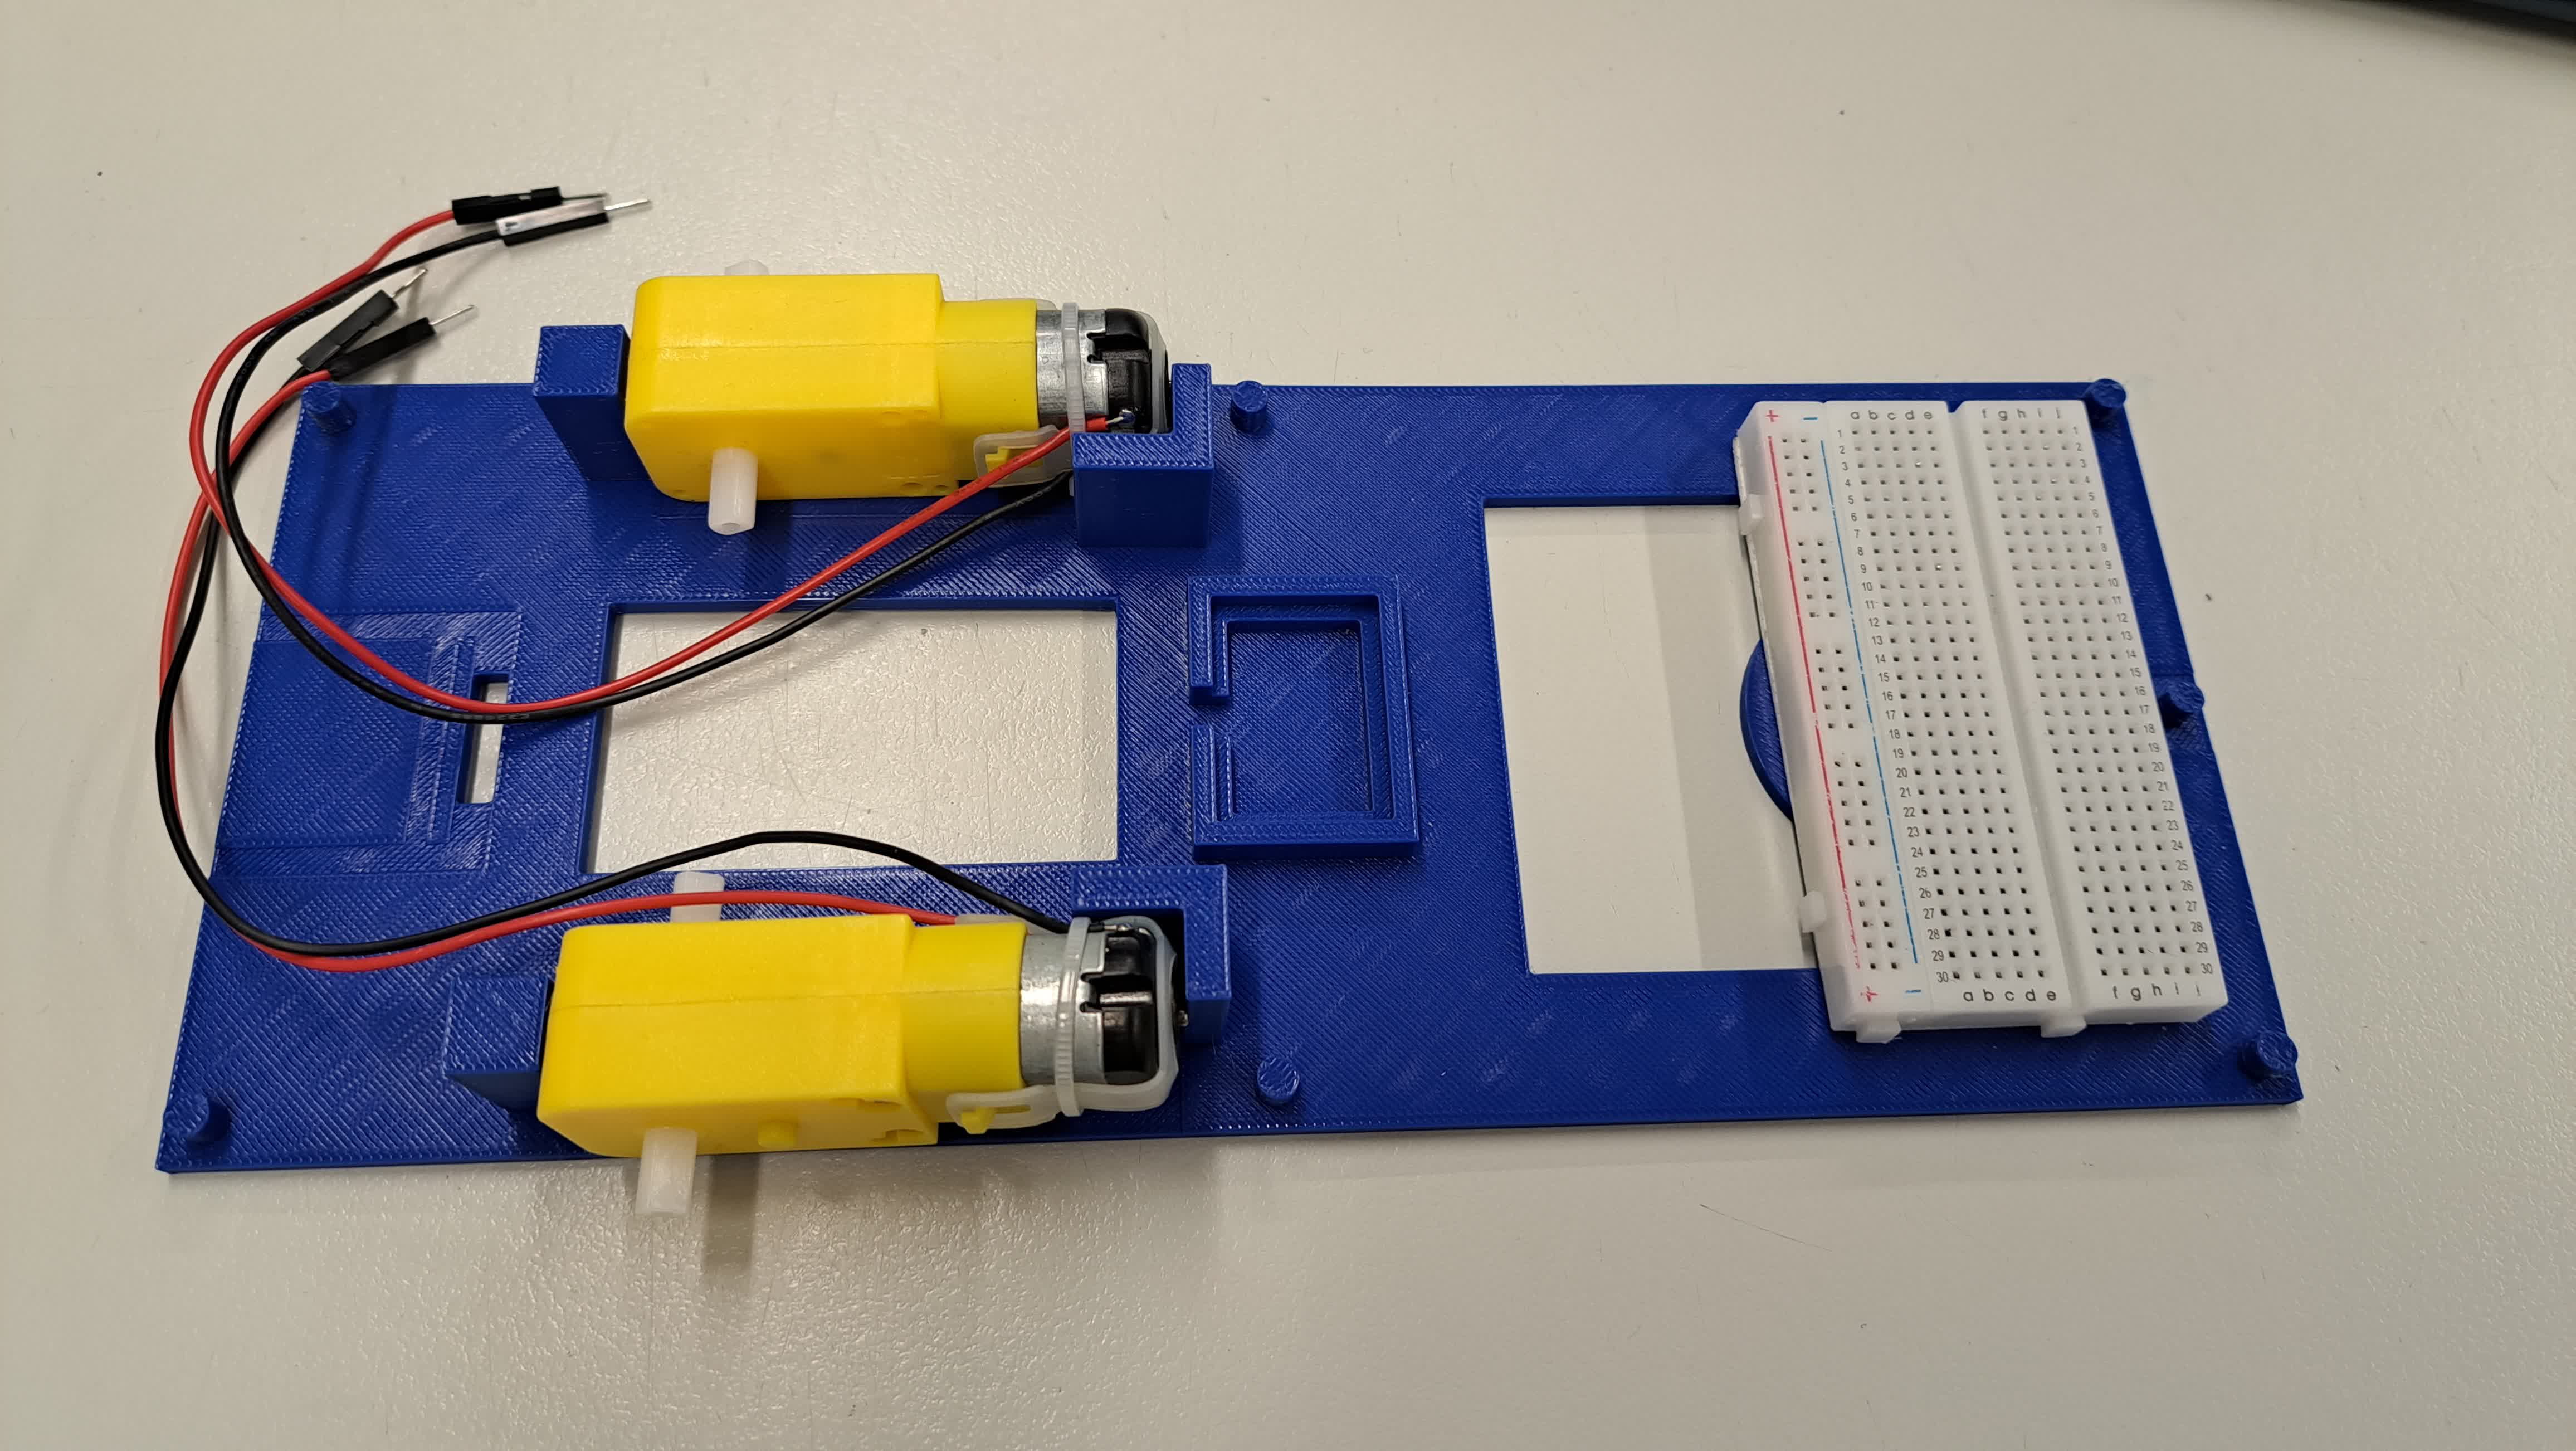
\includegraphics[width=\imagewidth]{IMG_1003}
% \end{figure}

\begin{figure}[H]
	\begin{subfigure}{0.95\imagewidth}
		\centering
		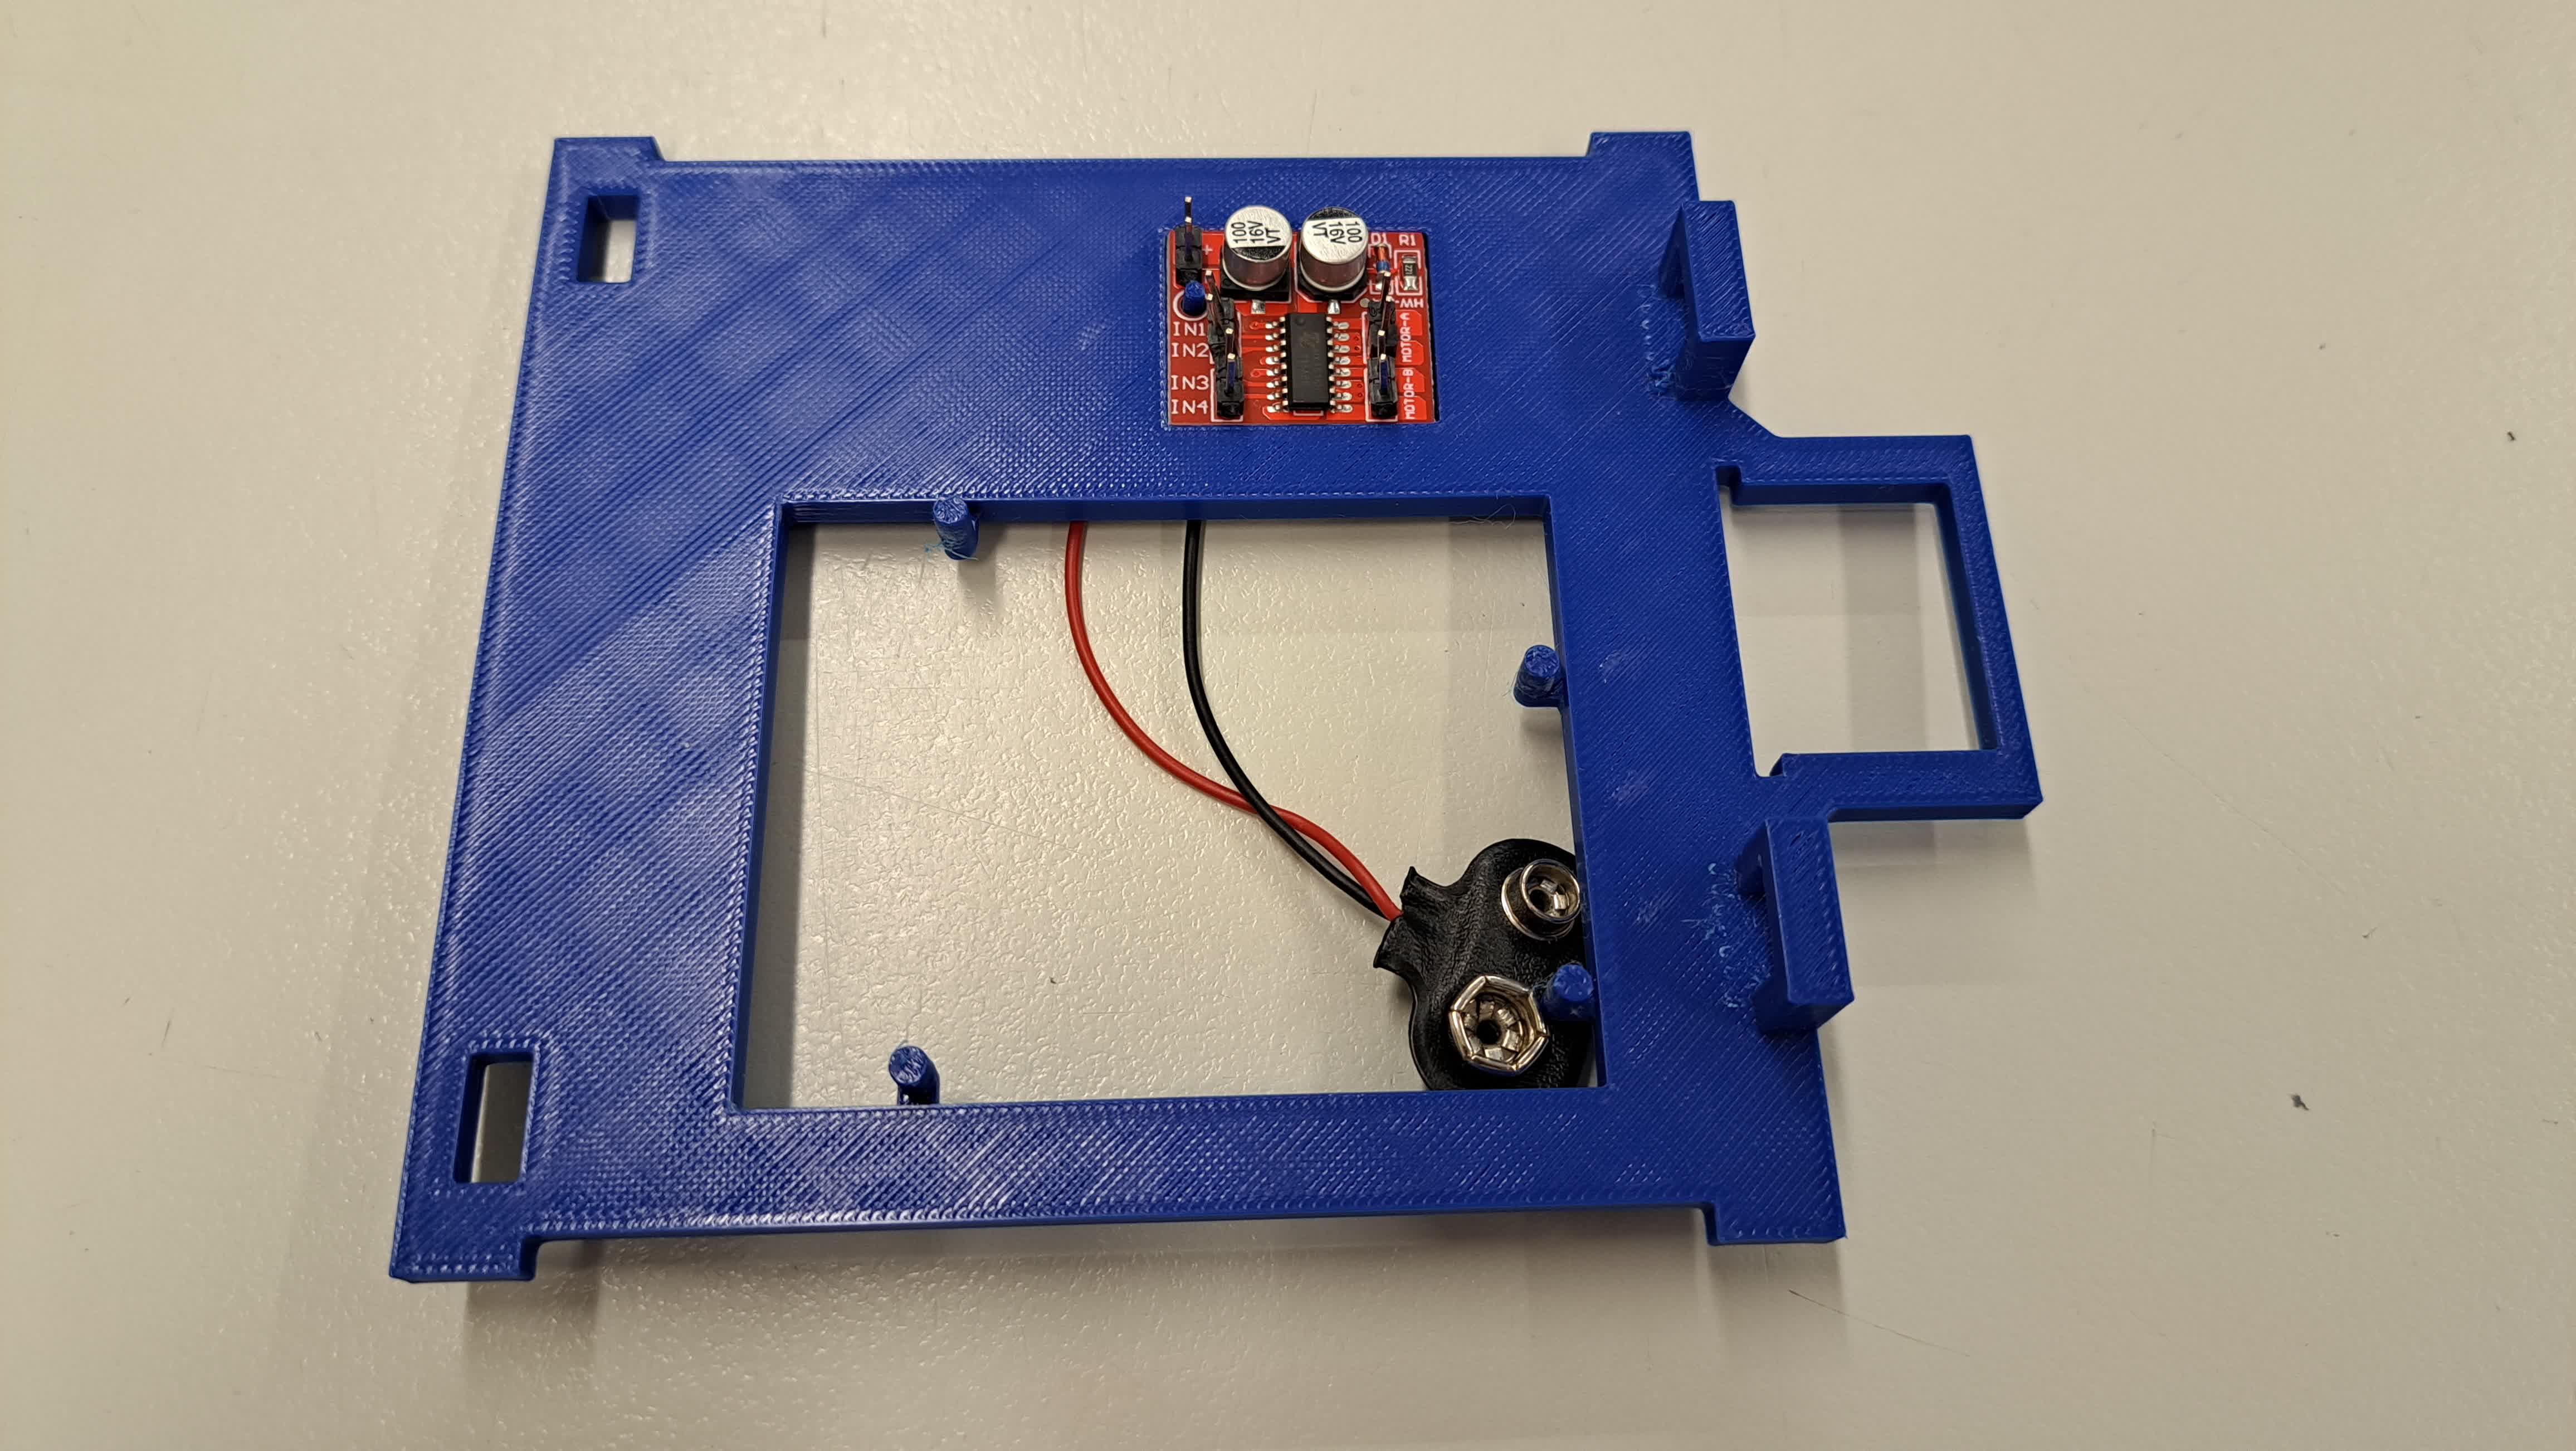
\includegraphics[width=0.9\imagewidth]{IMG_1004}
		\caption{Mittelplatte mit H-Brücke}
		\label{fig:1}
	\end{subfigure}
	\begin{subfigure}{0.95\imagewidth}
		\centering
		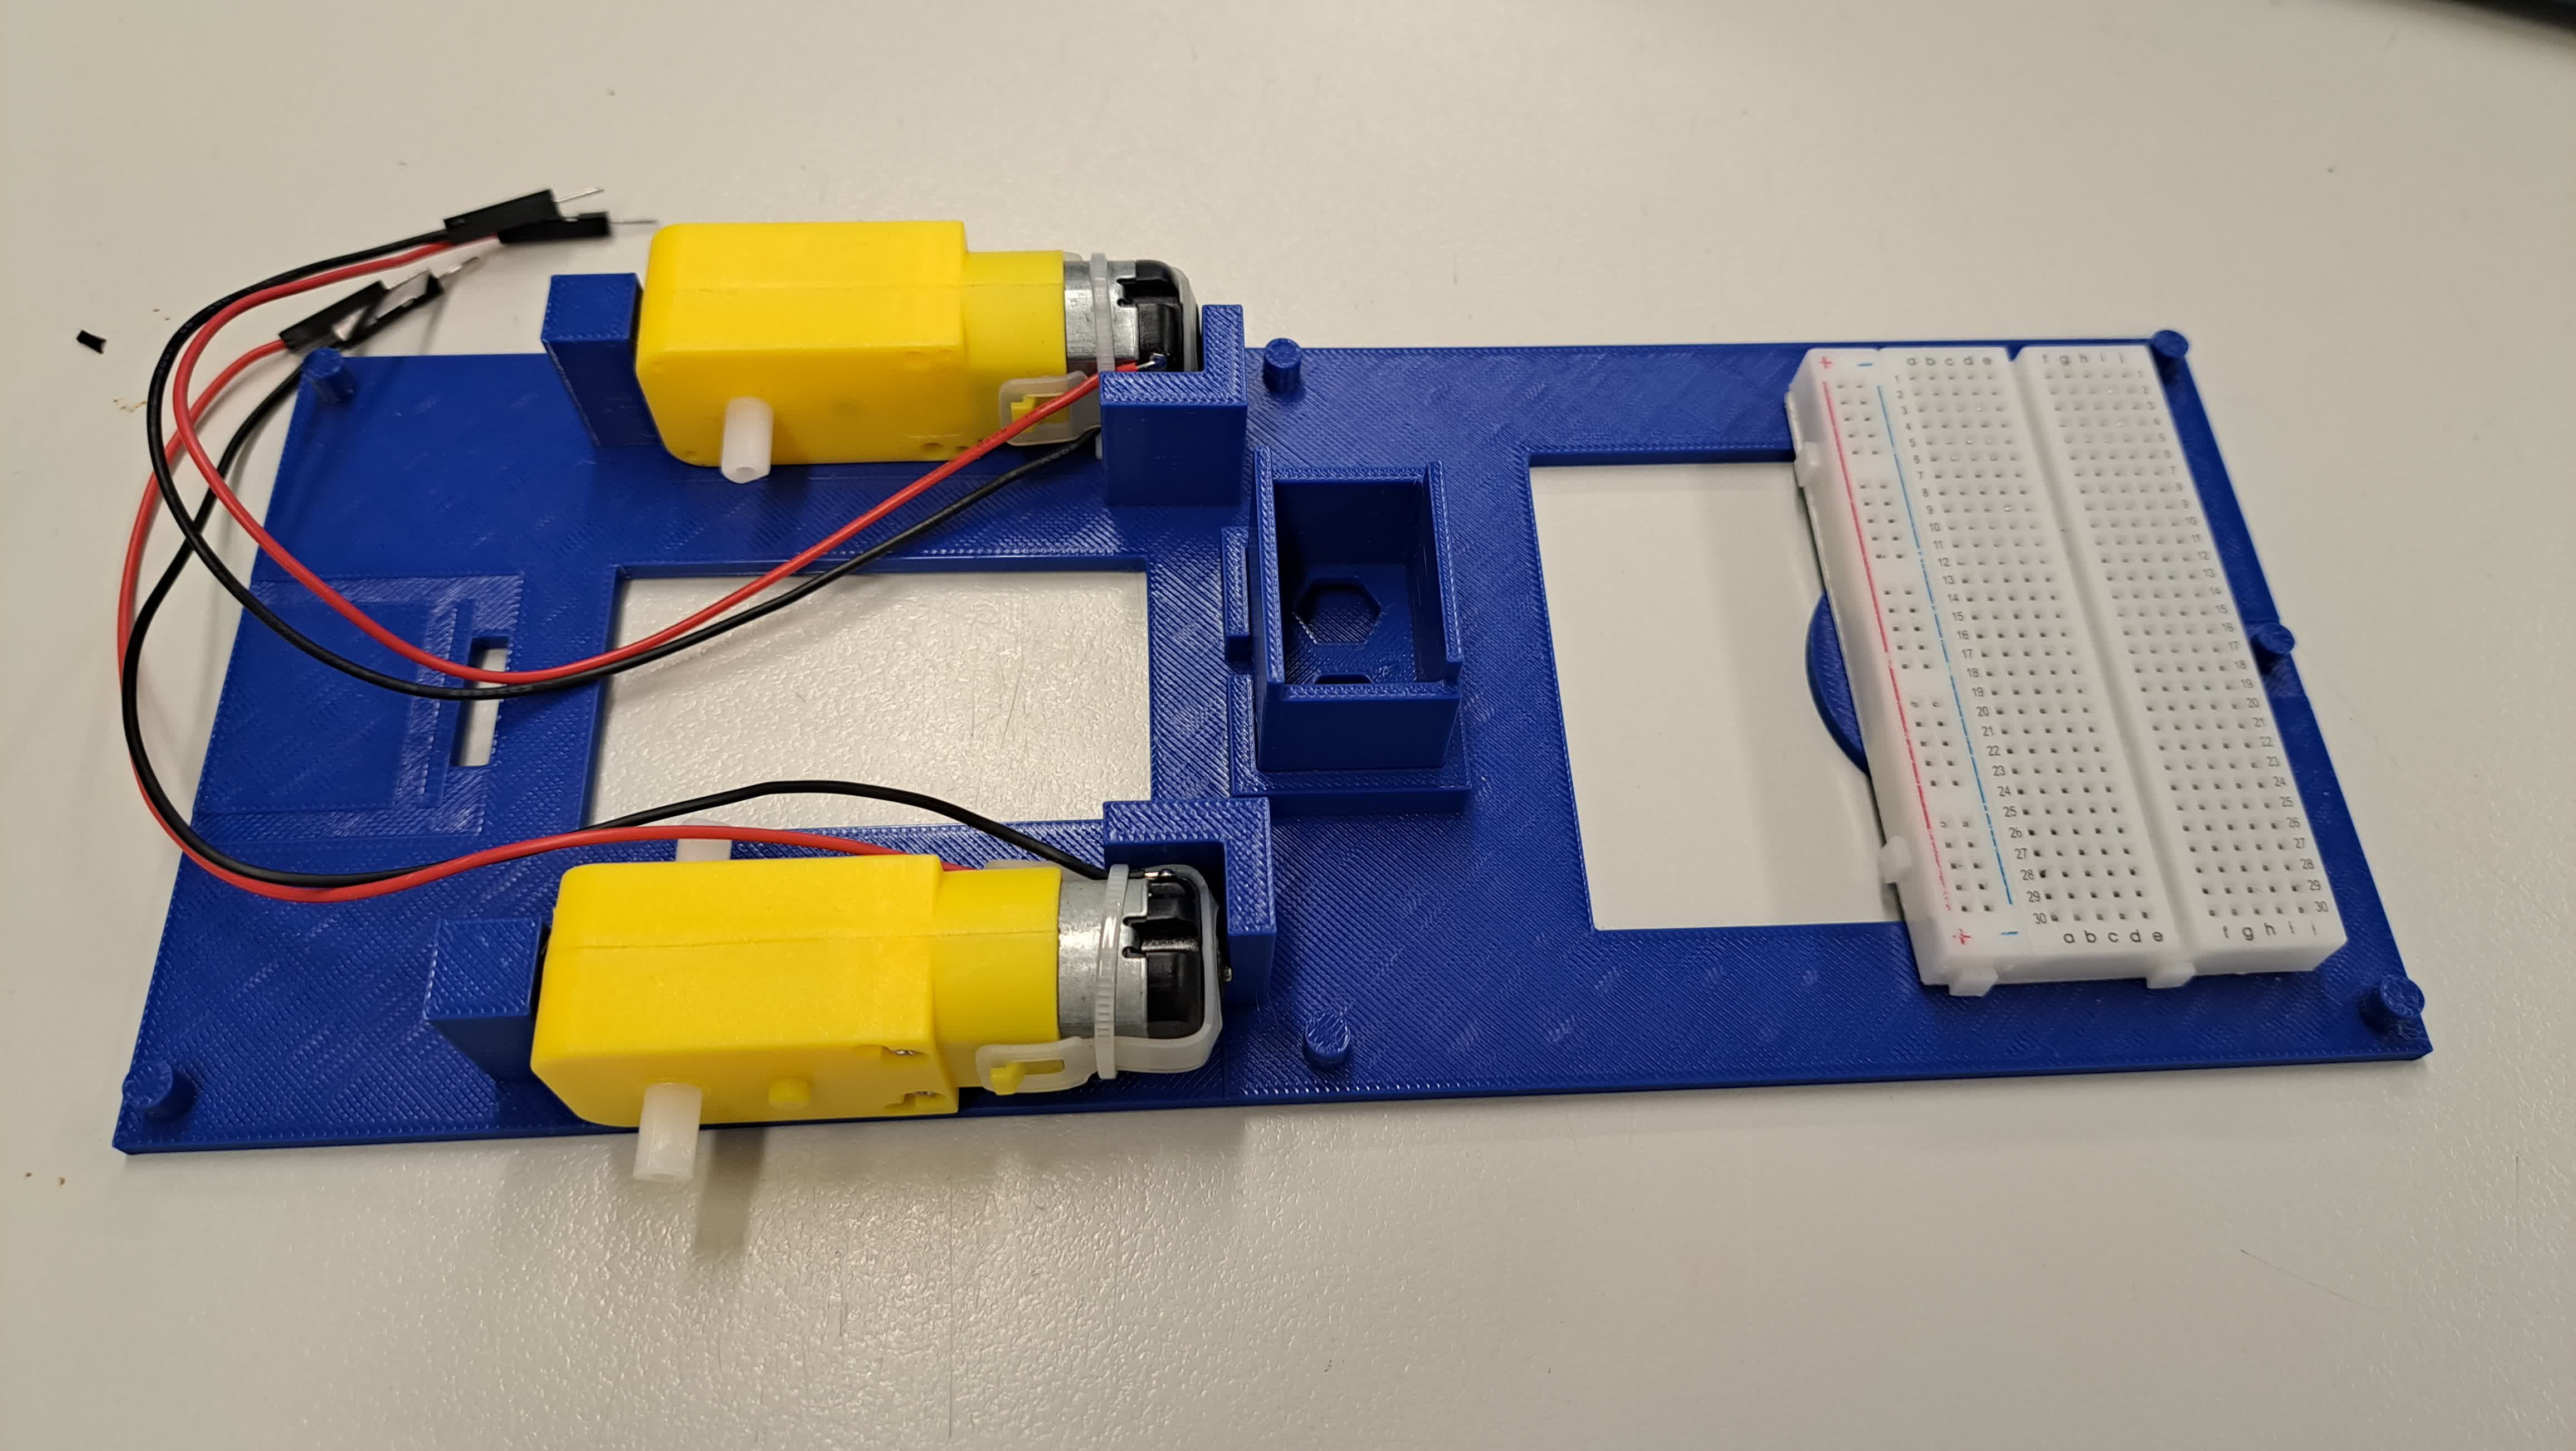
\includegraphics[width=0.9\imagewidth]{IMG_1005}
		\caption{Motoren und Breadboard auf Bodenplatte}
		\label{fig:2}
	\end{subfigure}
	\caption{Mittelplatte und Bodenplatte}
\end{figure}

Als erstes wird die H-Brücke in die Mittelplatte eingesetzt wie in Bild \ref{fig:1} zu sehen ist. Dazu wird die H-Brücke auf die Halterung gesteckt und die Kabel durch die Löcher geführt.

Danach werden die T-Motoren auf der Grundplatte eingesetzt und das Breadboard vorne auf die Mittelplatte geklebt wie in Bild \ref{fig:2} zu sehen ist.

\begin{figure}[H]
	\centering
	\begin{subfigure}{0.95\imagewidth}
		\centering
		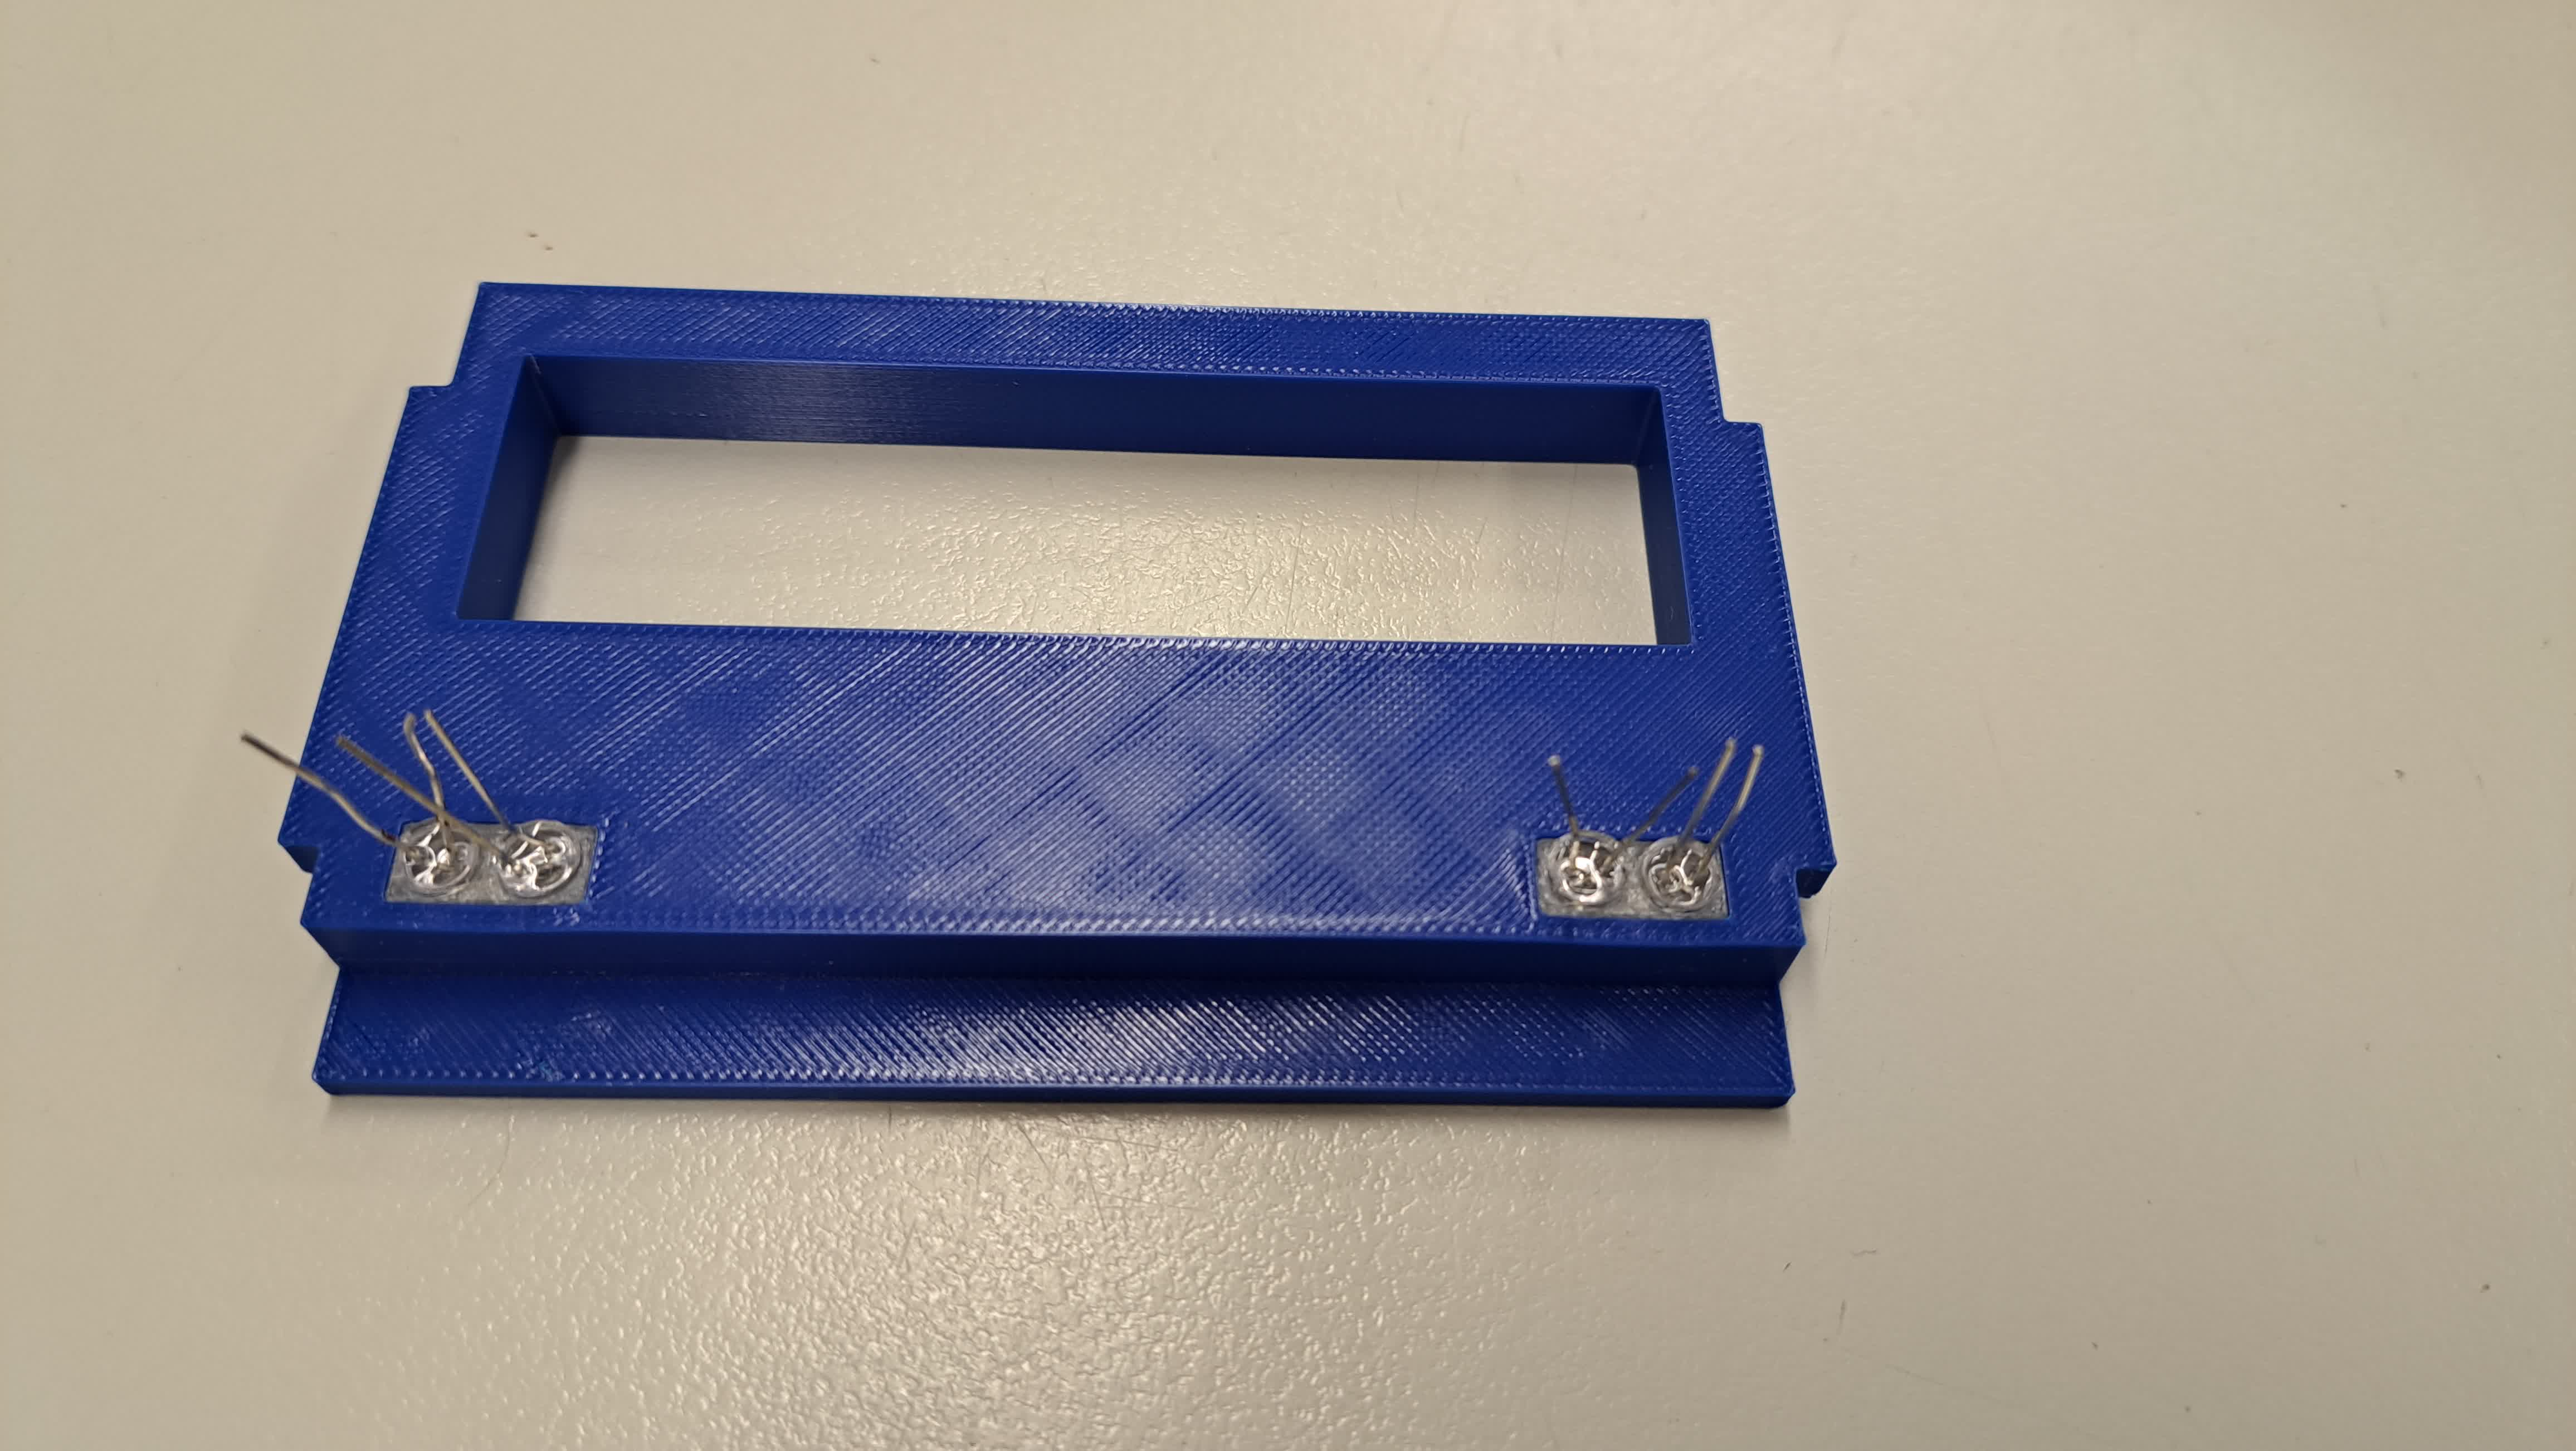
\includegraphics[width=0.9\imagewidth]{IMG_1006}
		\caption{Rückseite}
		\label{fig:3}
	\end{subfigure}
	\begin{subfigure}{0.95\imagewidth}
		\centering
		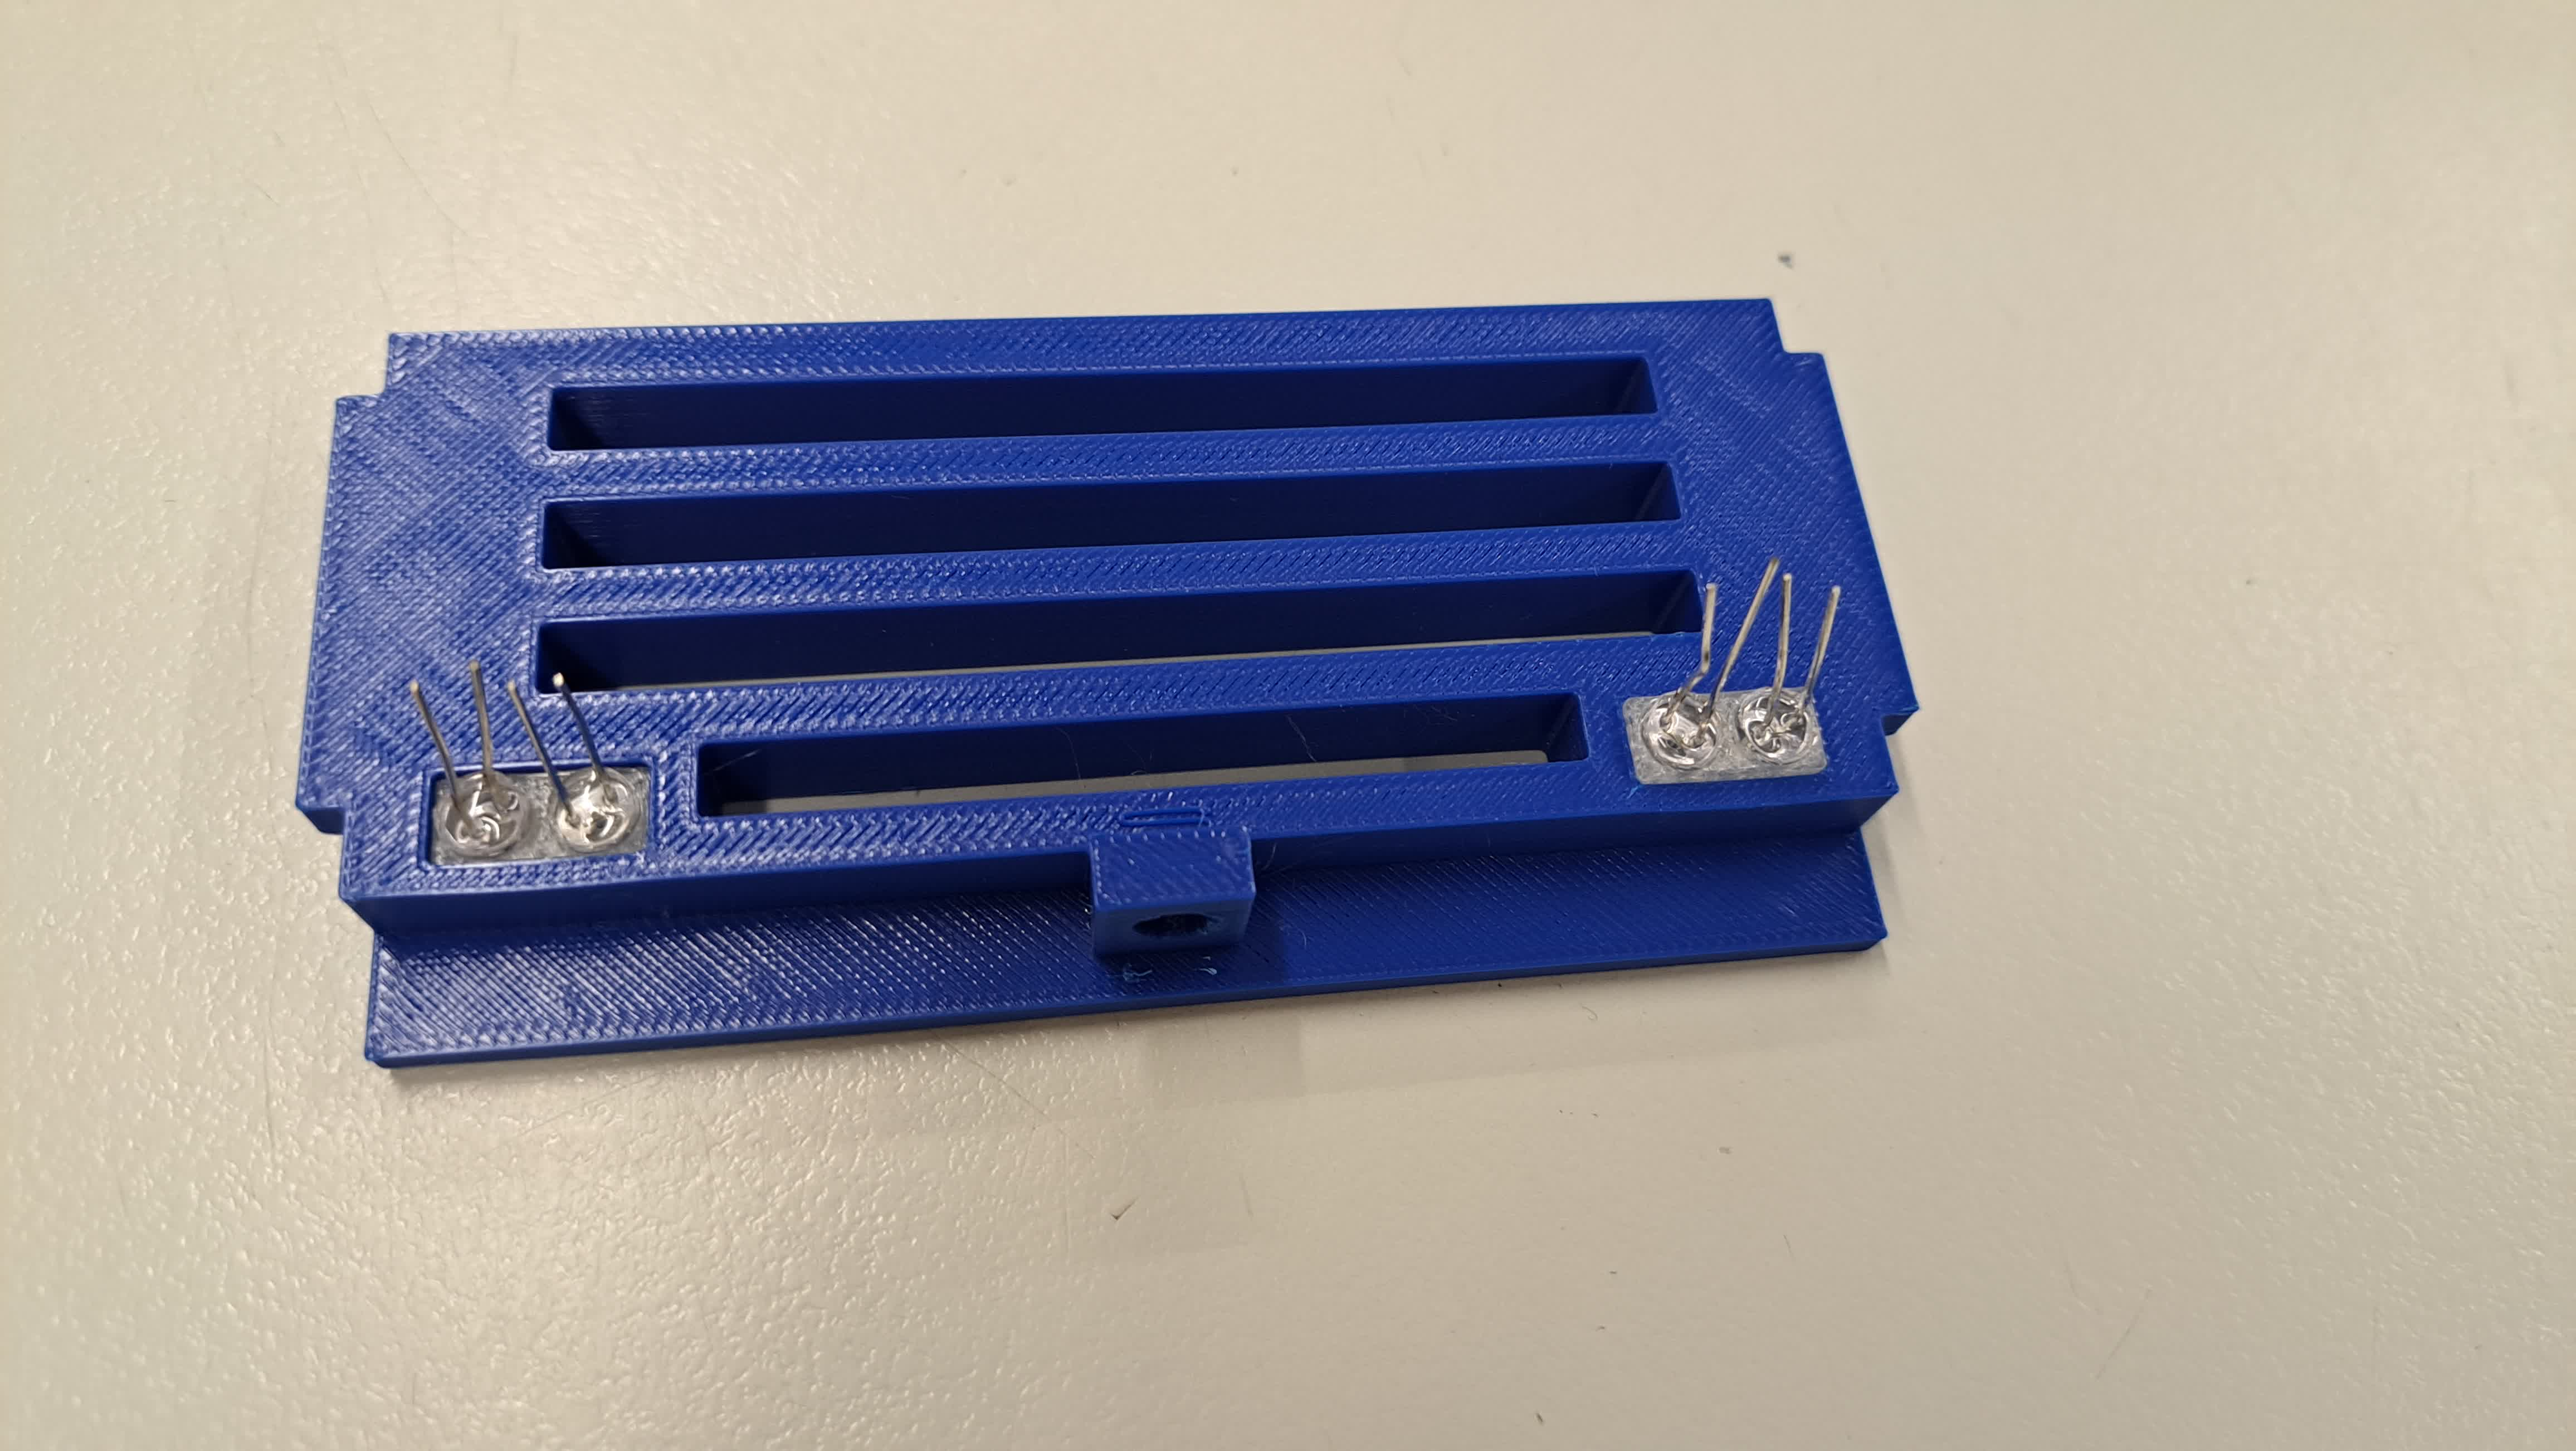
\includegraphics[width=0.9\imagewidth]{IMG_1007}
		\caption{Vorderseite}
		\label{fig:4}
	\end{subfigure}
	\caption{Front- und Rückseite mit LEDs}
\end{figure}

Anschließend werden die LEDs in die Front- und Rückseite eingesetzt wie in Bild \ref{fig:3} und Bild \ref{fig:4} zu sehen ist. Dabei packt ihr jeweils eine gelbe LED in die Außenseite jedes Scheinwerfers und eine weiße LED in die Innenseite, bei der Vorderseite, und eine rote LED in die Innenseite, bei der Rückseite.

\begin{figure}[H]
	\centering
	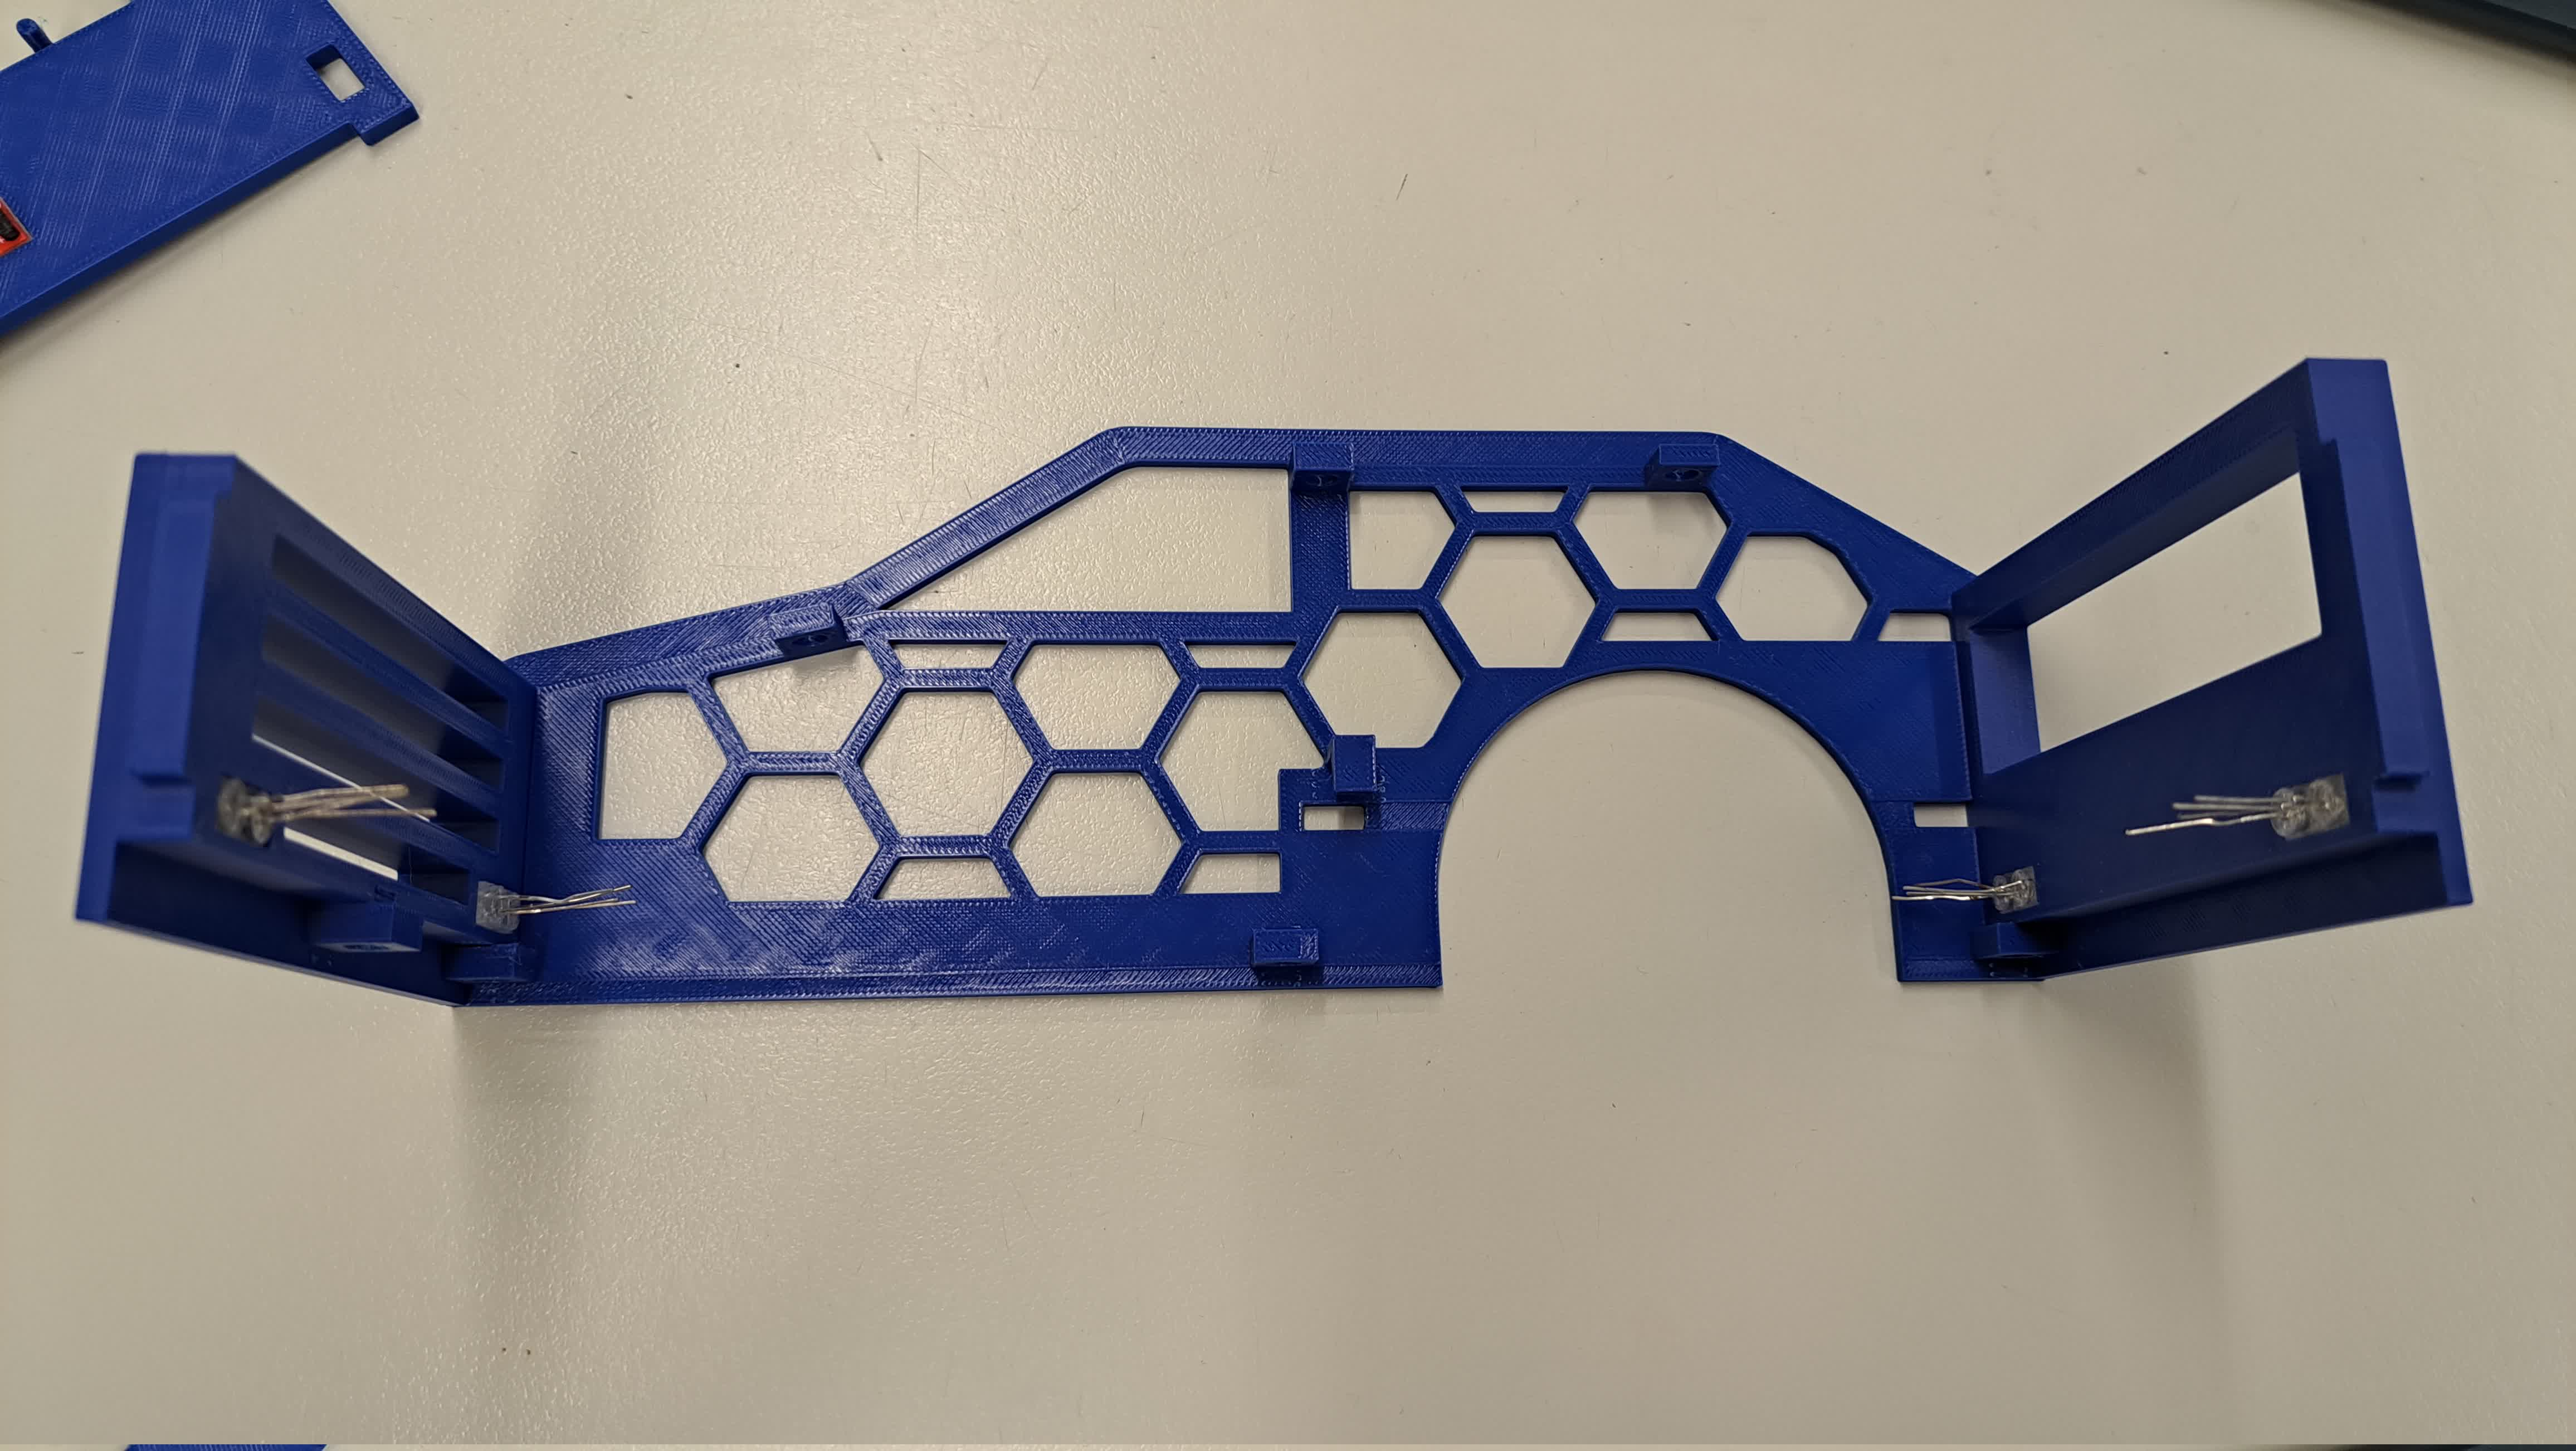
\includegraphics[width=0.9\imagewidth]{IMG_1008}
	\caption{Außenverkleidung}
	\label{fig:5}
\end{figure}

Danach steckt ihr die Front- und Rückseite in die Außenverkleidung wie in Bild \ref{fig:5} zu sehen ist.

\begin{figure}[H]
	\centering
	\begin{subfigure}{0.95\imagewidth}
		\centering
		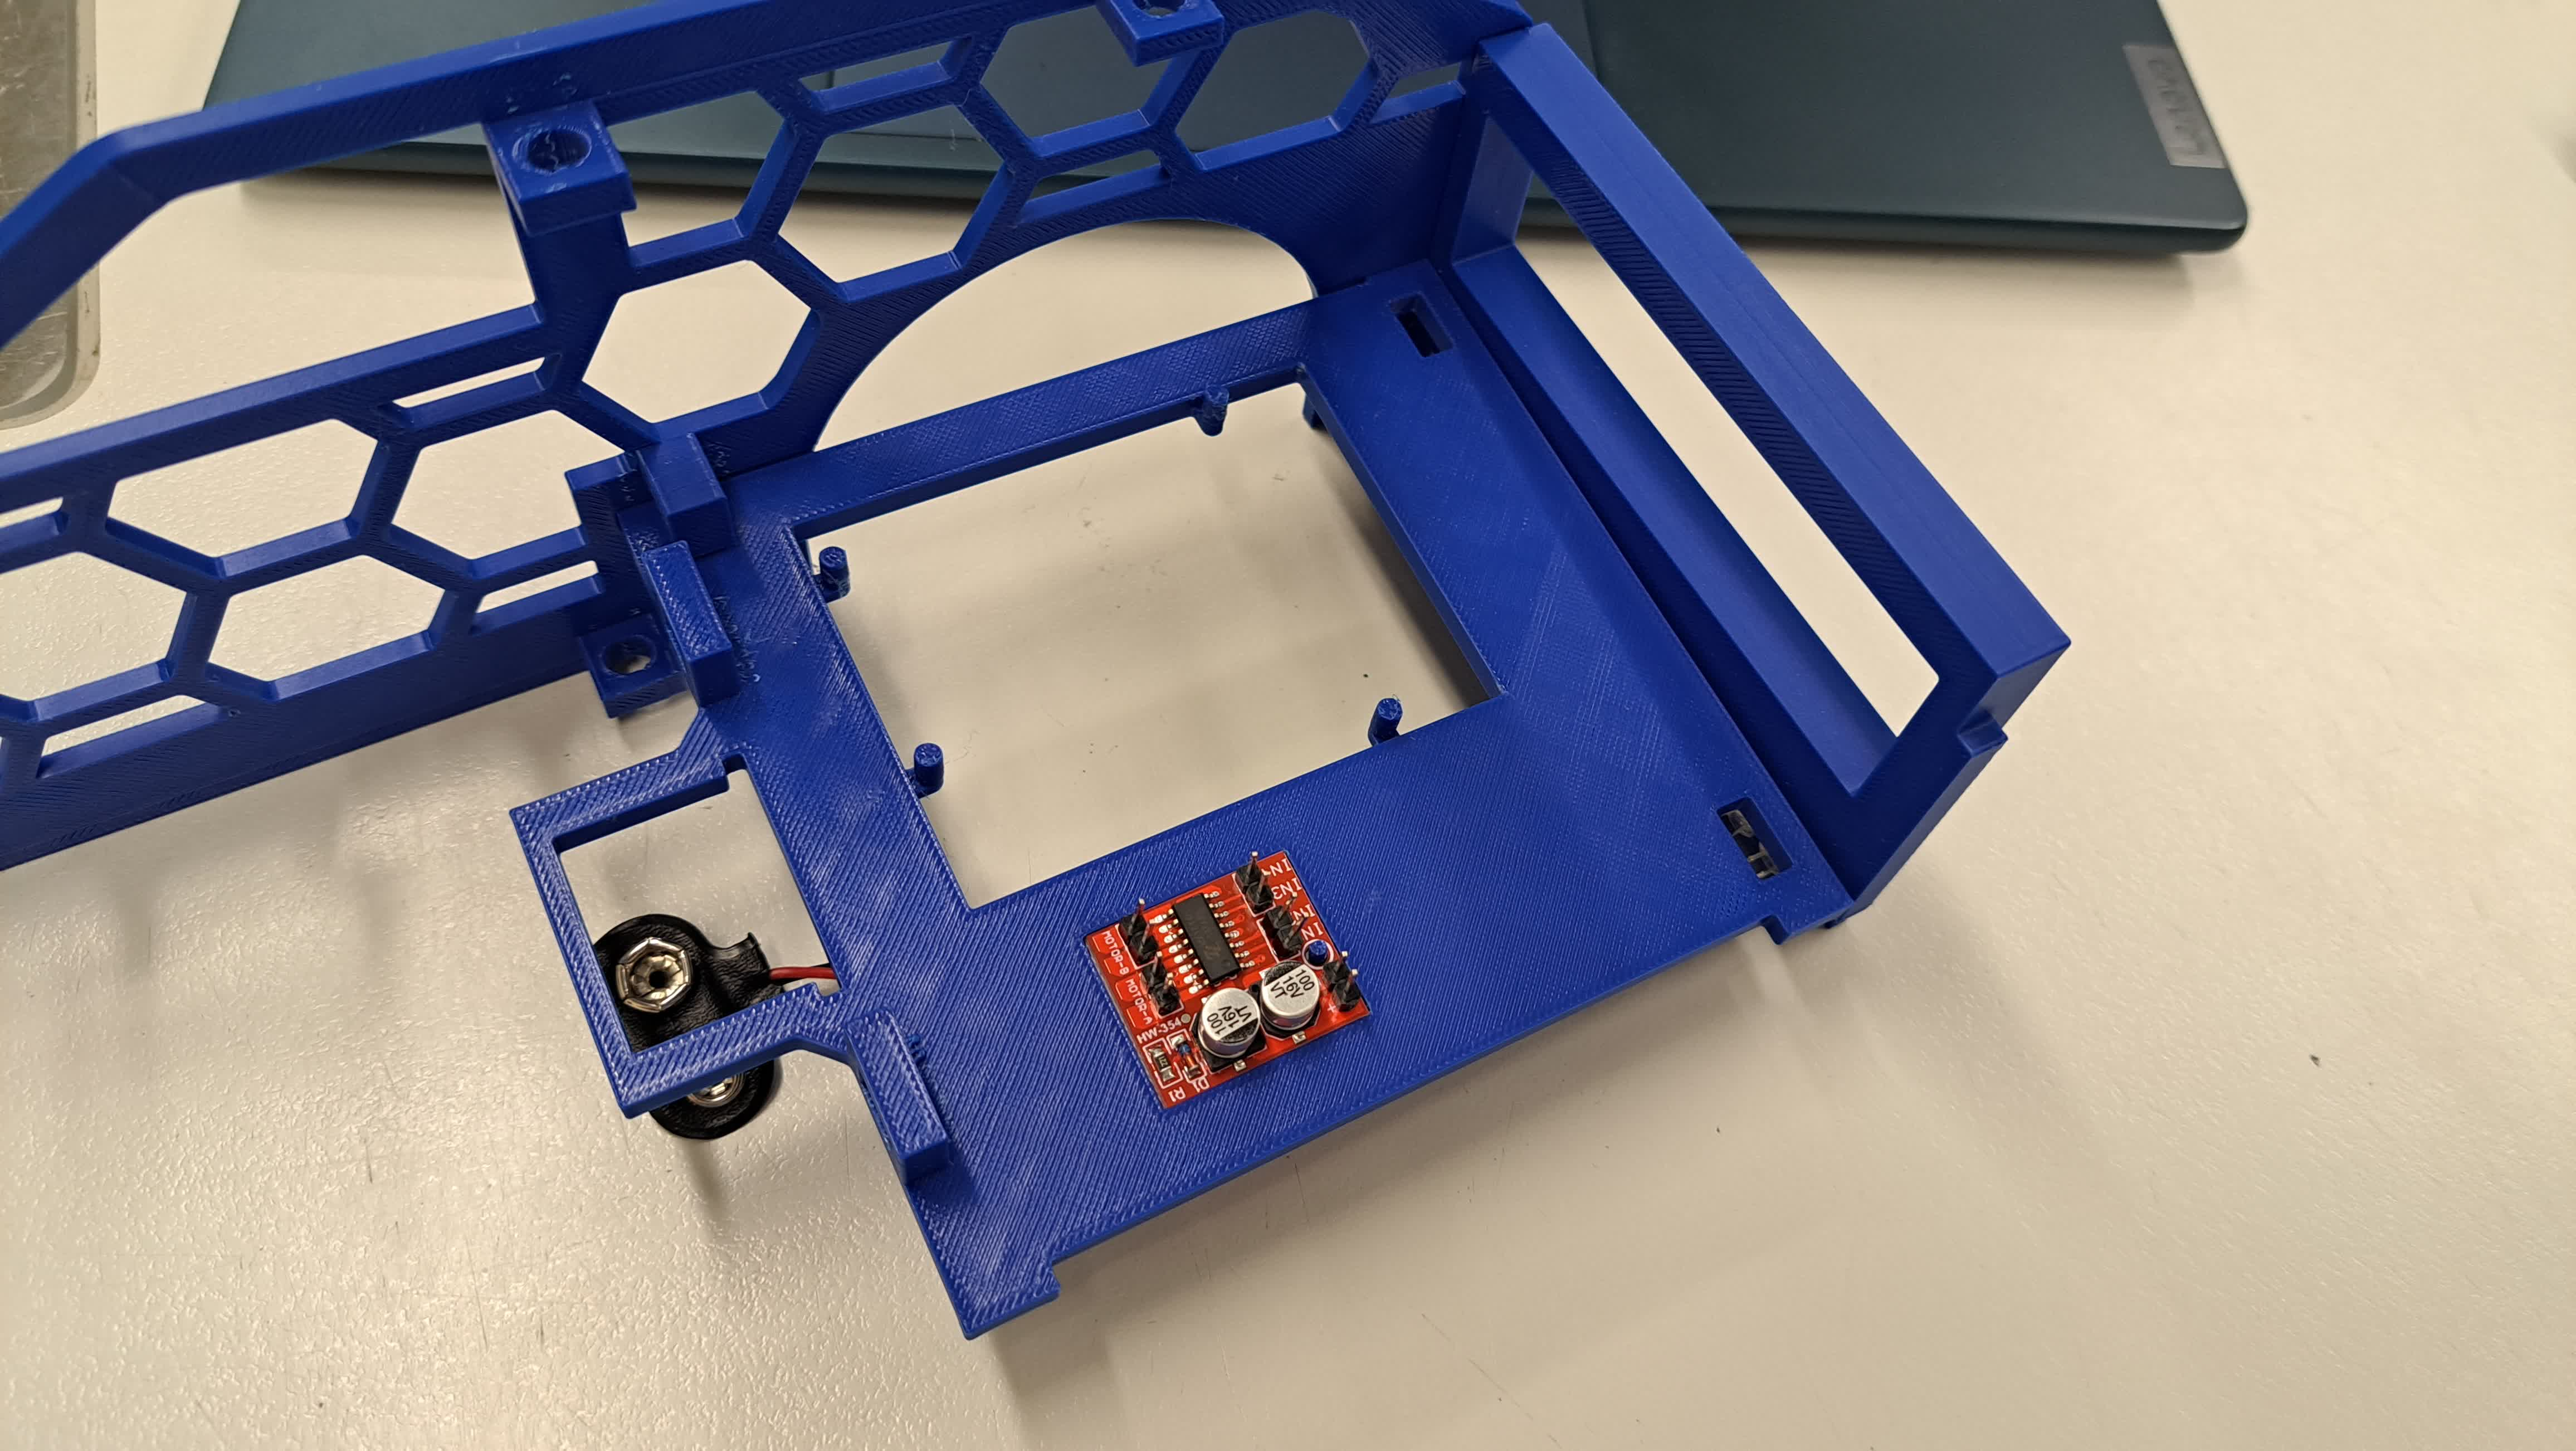
\includegraphics[width=0.9\imagewidth]{IMG_1010}
		\caption{Von oben}
		\label{fig:6}
	\end{subfigure}
	\begin{subfigure}{0.95\imagewidth}
		\centering
		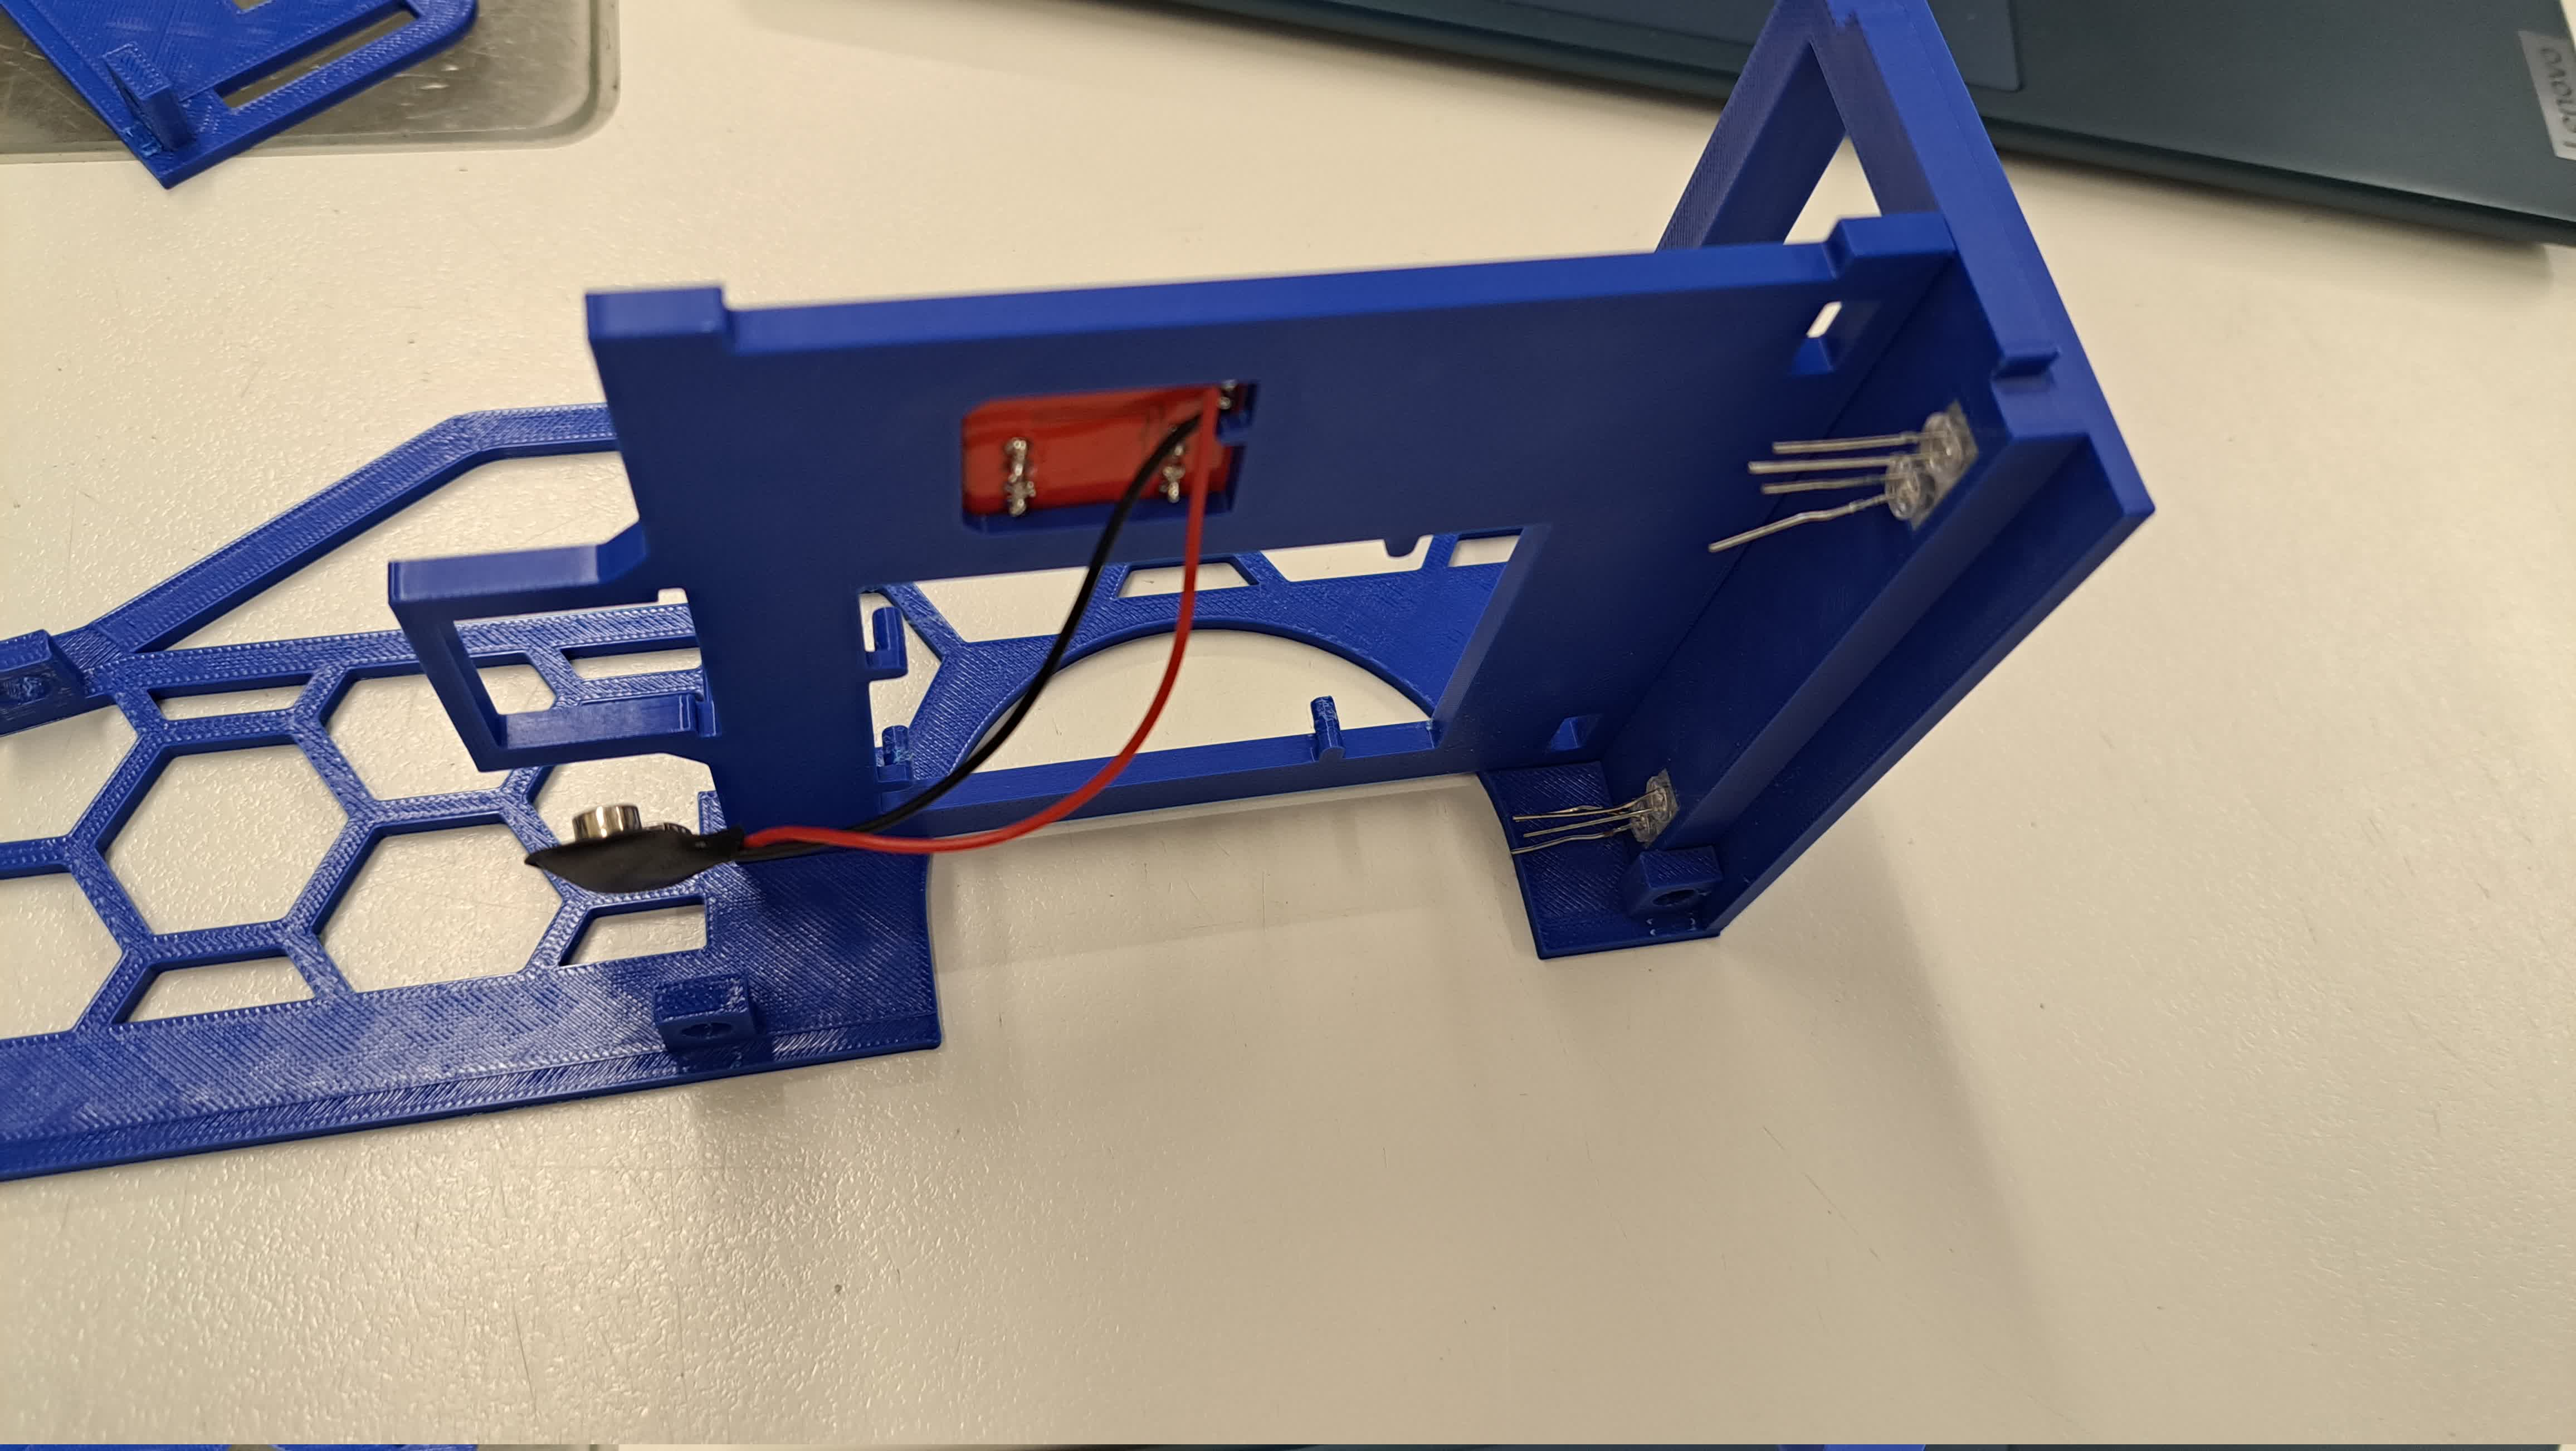
\includegraphics[width=0.9\imagewidth]{IMG_1009}
		\caption{Von unten}
		\label{fig:7}
	\end{subfigure}
	\caption{Außenverkleidung von oben und unten}
\end{figure}

Anschließend könnt ihr die Mittelplatte in die Außenwand packen wie in Bild \ref{fig:6} und Bild \ref{fig:7} zu sehen ist. Zusätzlich schließt ihr an jedes Ende der LEDs an der Rückseite ein Female-Male Kabel und führt diese unter Mittelplatte nach Vorne weiter. Damit ihr besser sehen könnt, welches Kabel für was benutzt wird, solltet ihr für den Minuspol der Leds alle die selbe Farbe benutzen, z.B. schwarz, und für den Pluspol der Rücklichter eine andere Farbe, z.B. rot, und für den Pluspol der Blinker eine andere Farbe, z.B. gelb.

\begin{figure}[H]
	\centering
	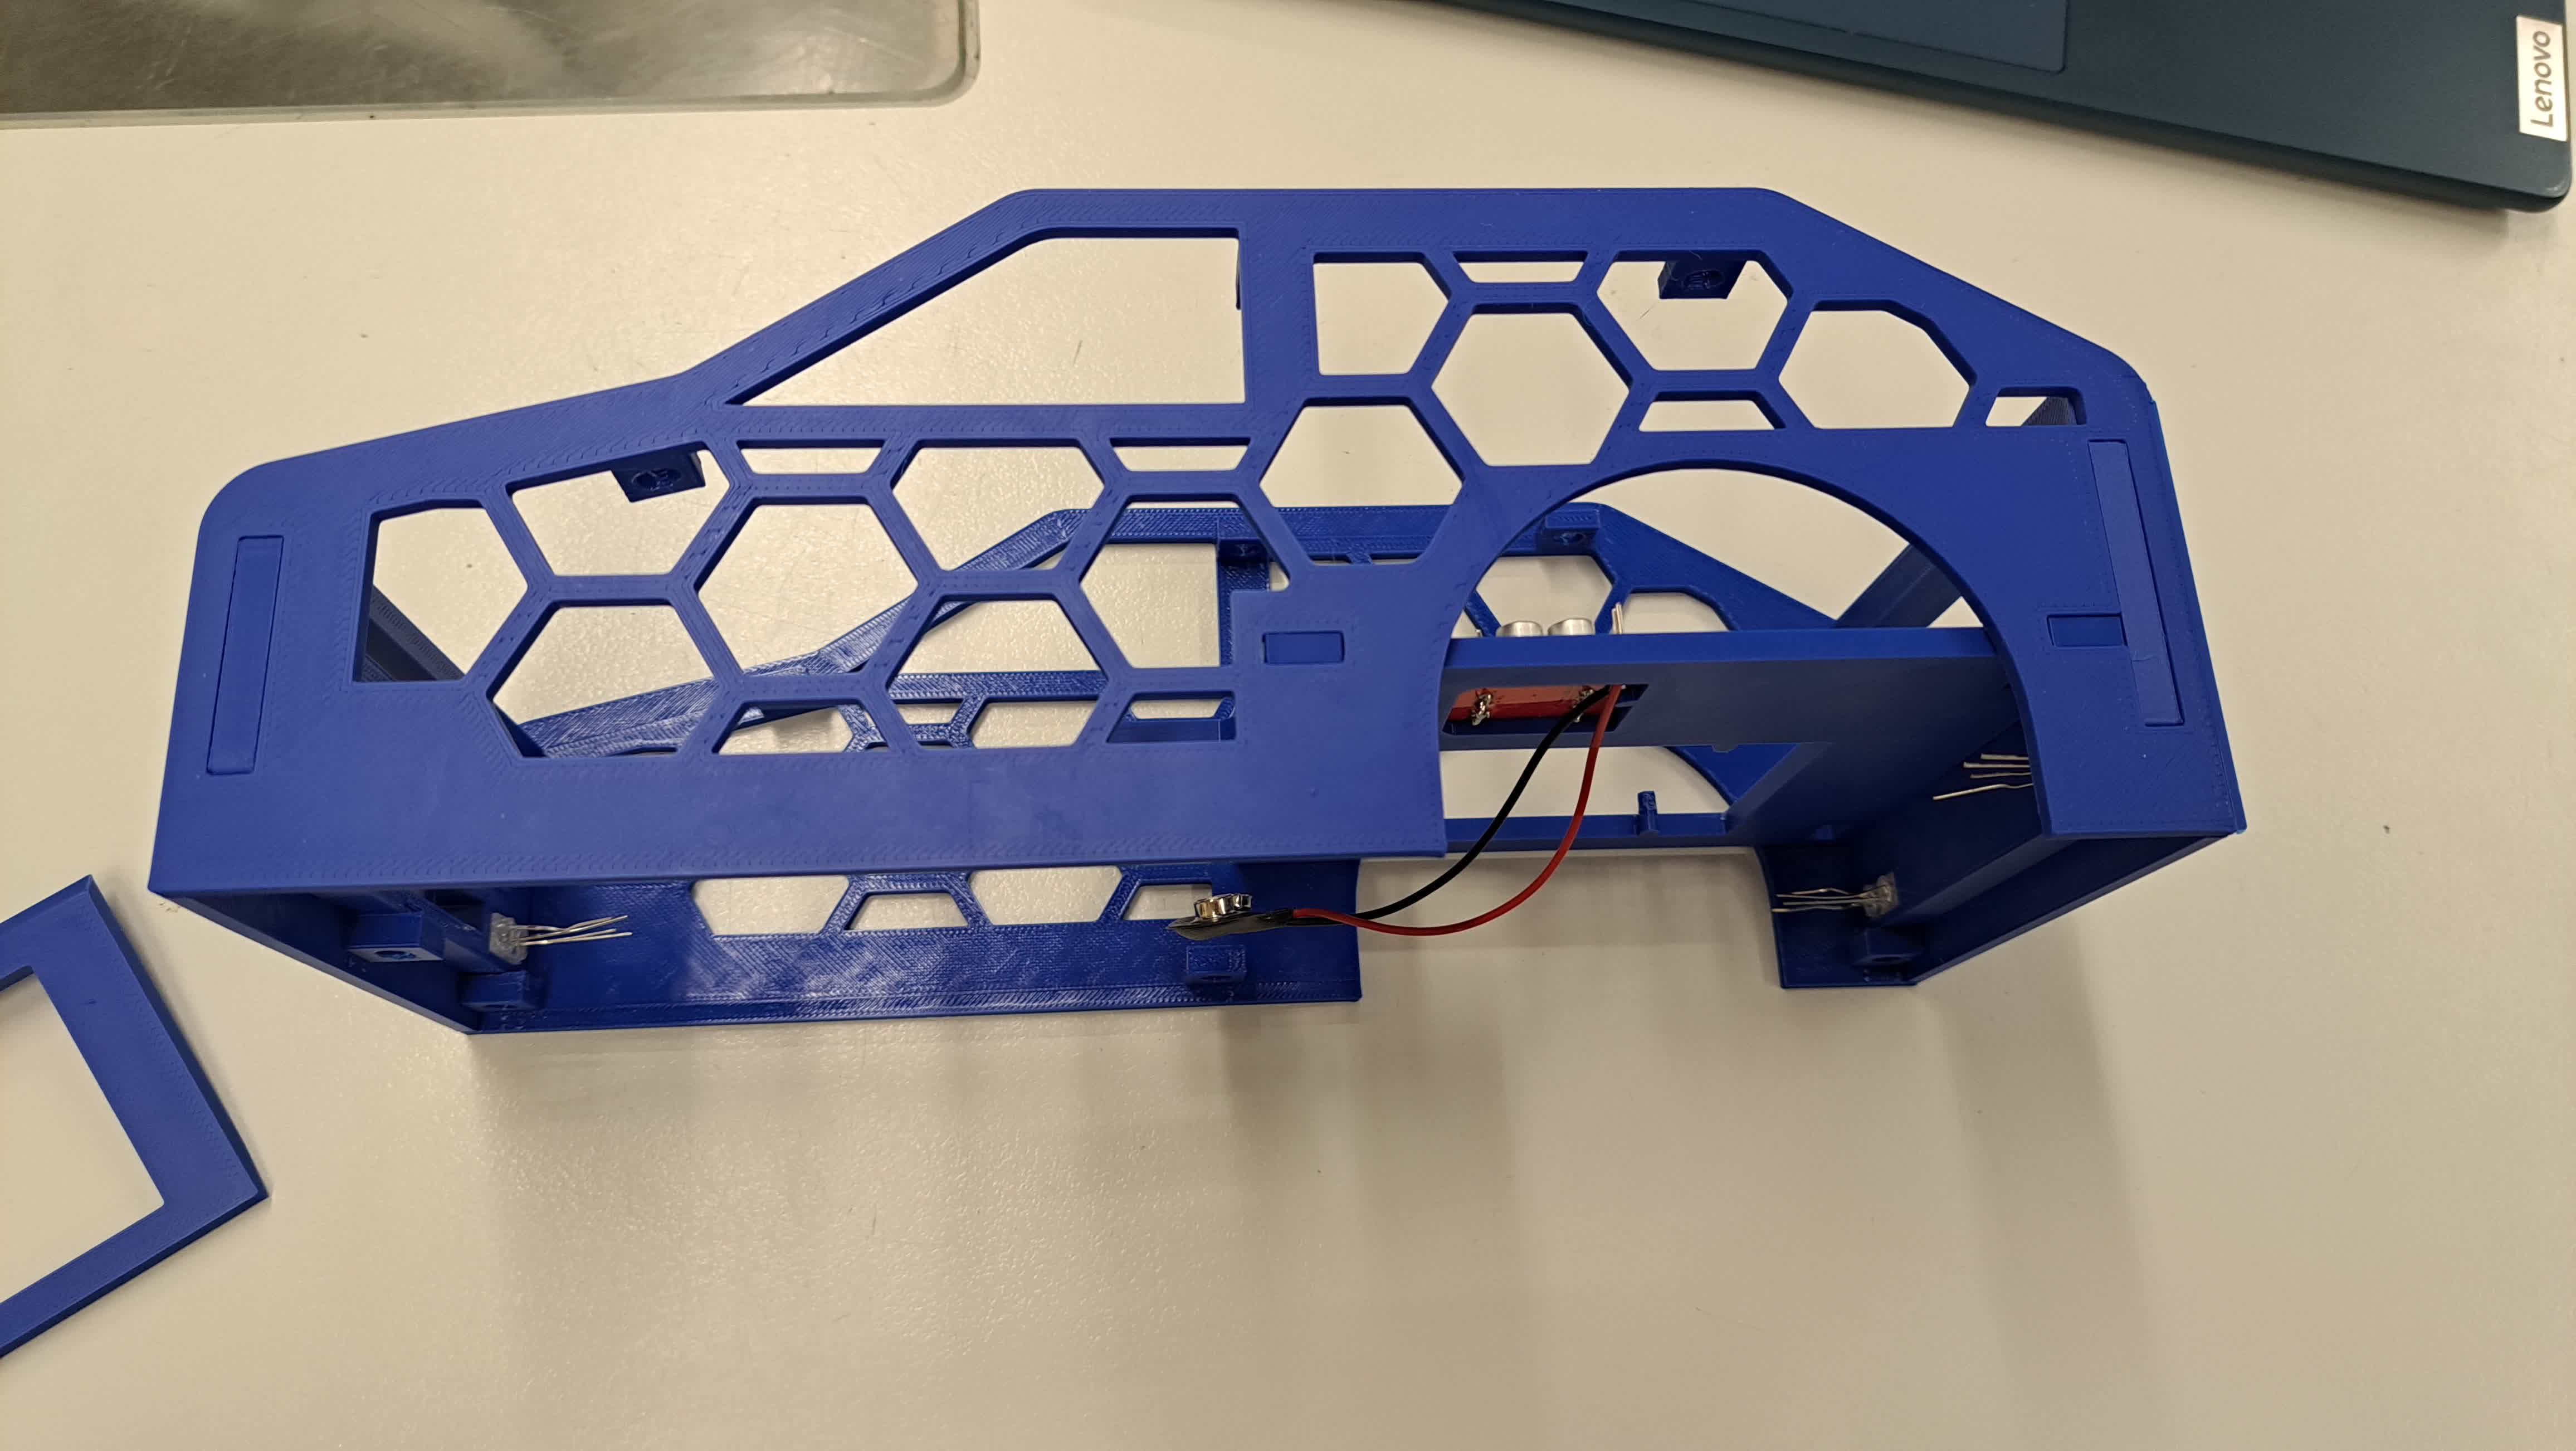
\includegraphics[width=\imagewidth]{IMG_1011}
	\caption{Außenverkleidung fertig}
	\label{fig:8}
\end{figure}

Danach könnt ihr die Außenverkleidung fertig zusammenbauen wie in Bild \ref{fig:8} zu sehen ist.

\begin{figure}[H]
	\begin{subfigure}{0.95\imagewidth}
		\centering
		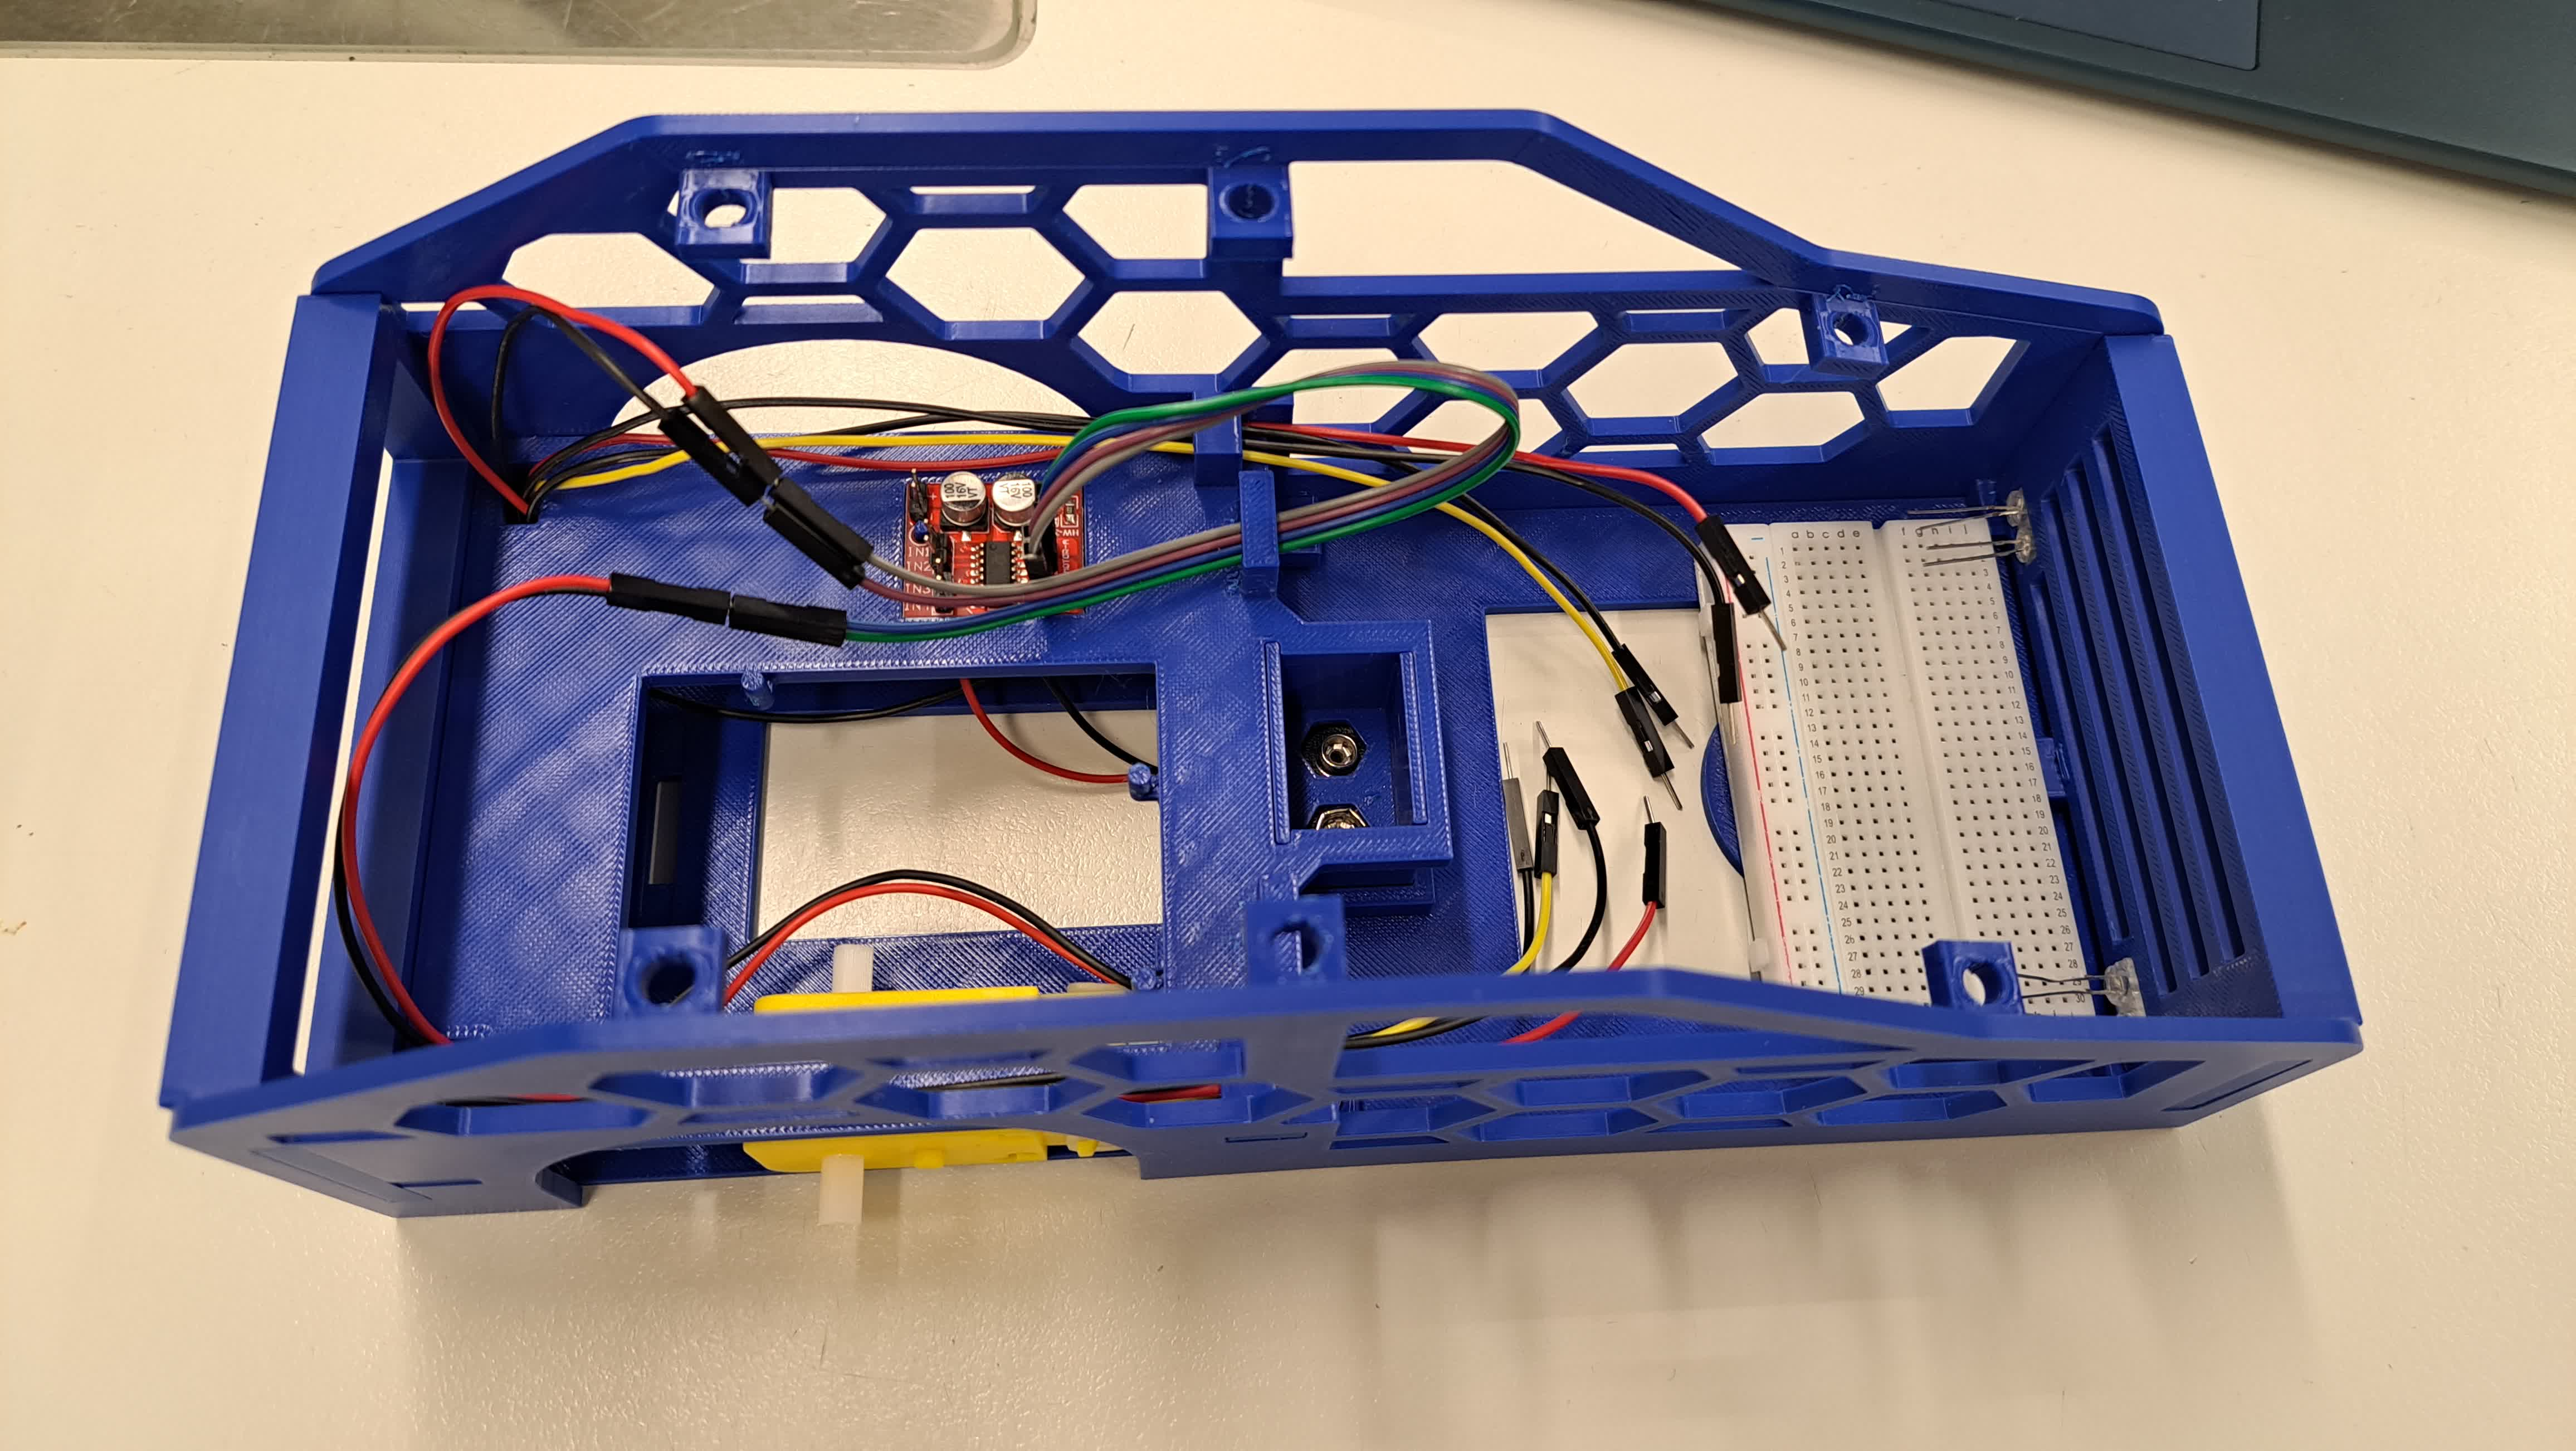
\includegraphics[width=0.9\imagewidth]{IMG_1013}
		\caption{Bodenplatte und Außenverkleidung}
		\label{fig:9}
	\end{subfigure}
	\begin{subfigure}{0.95\imagewidth}
		\centering
		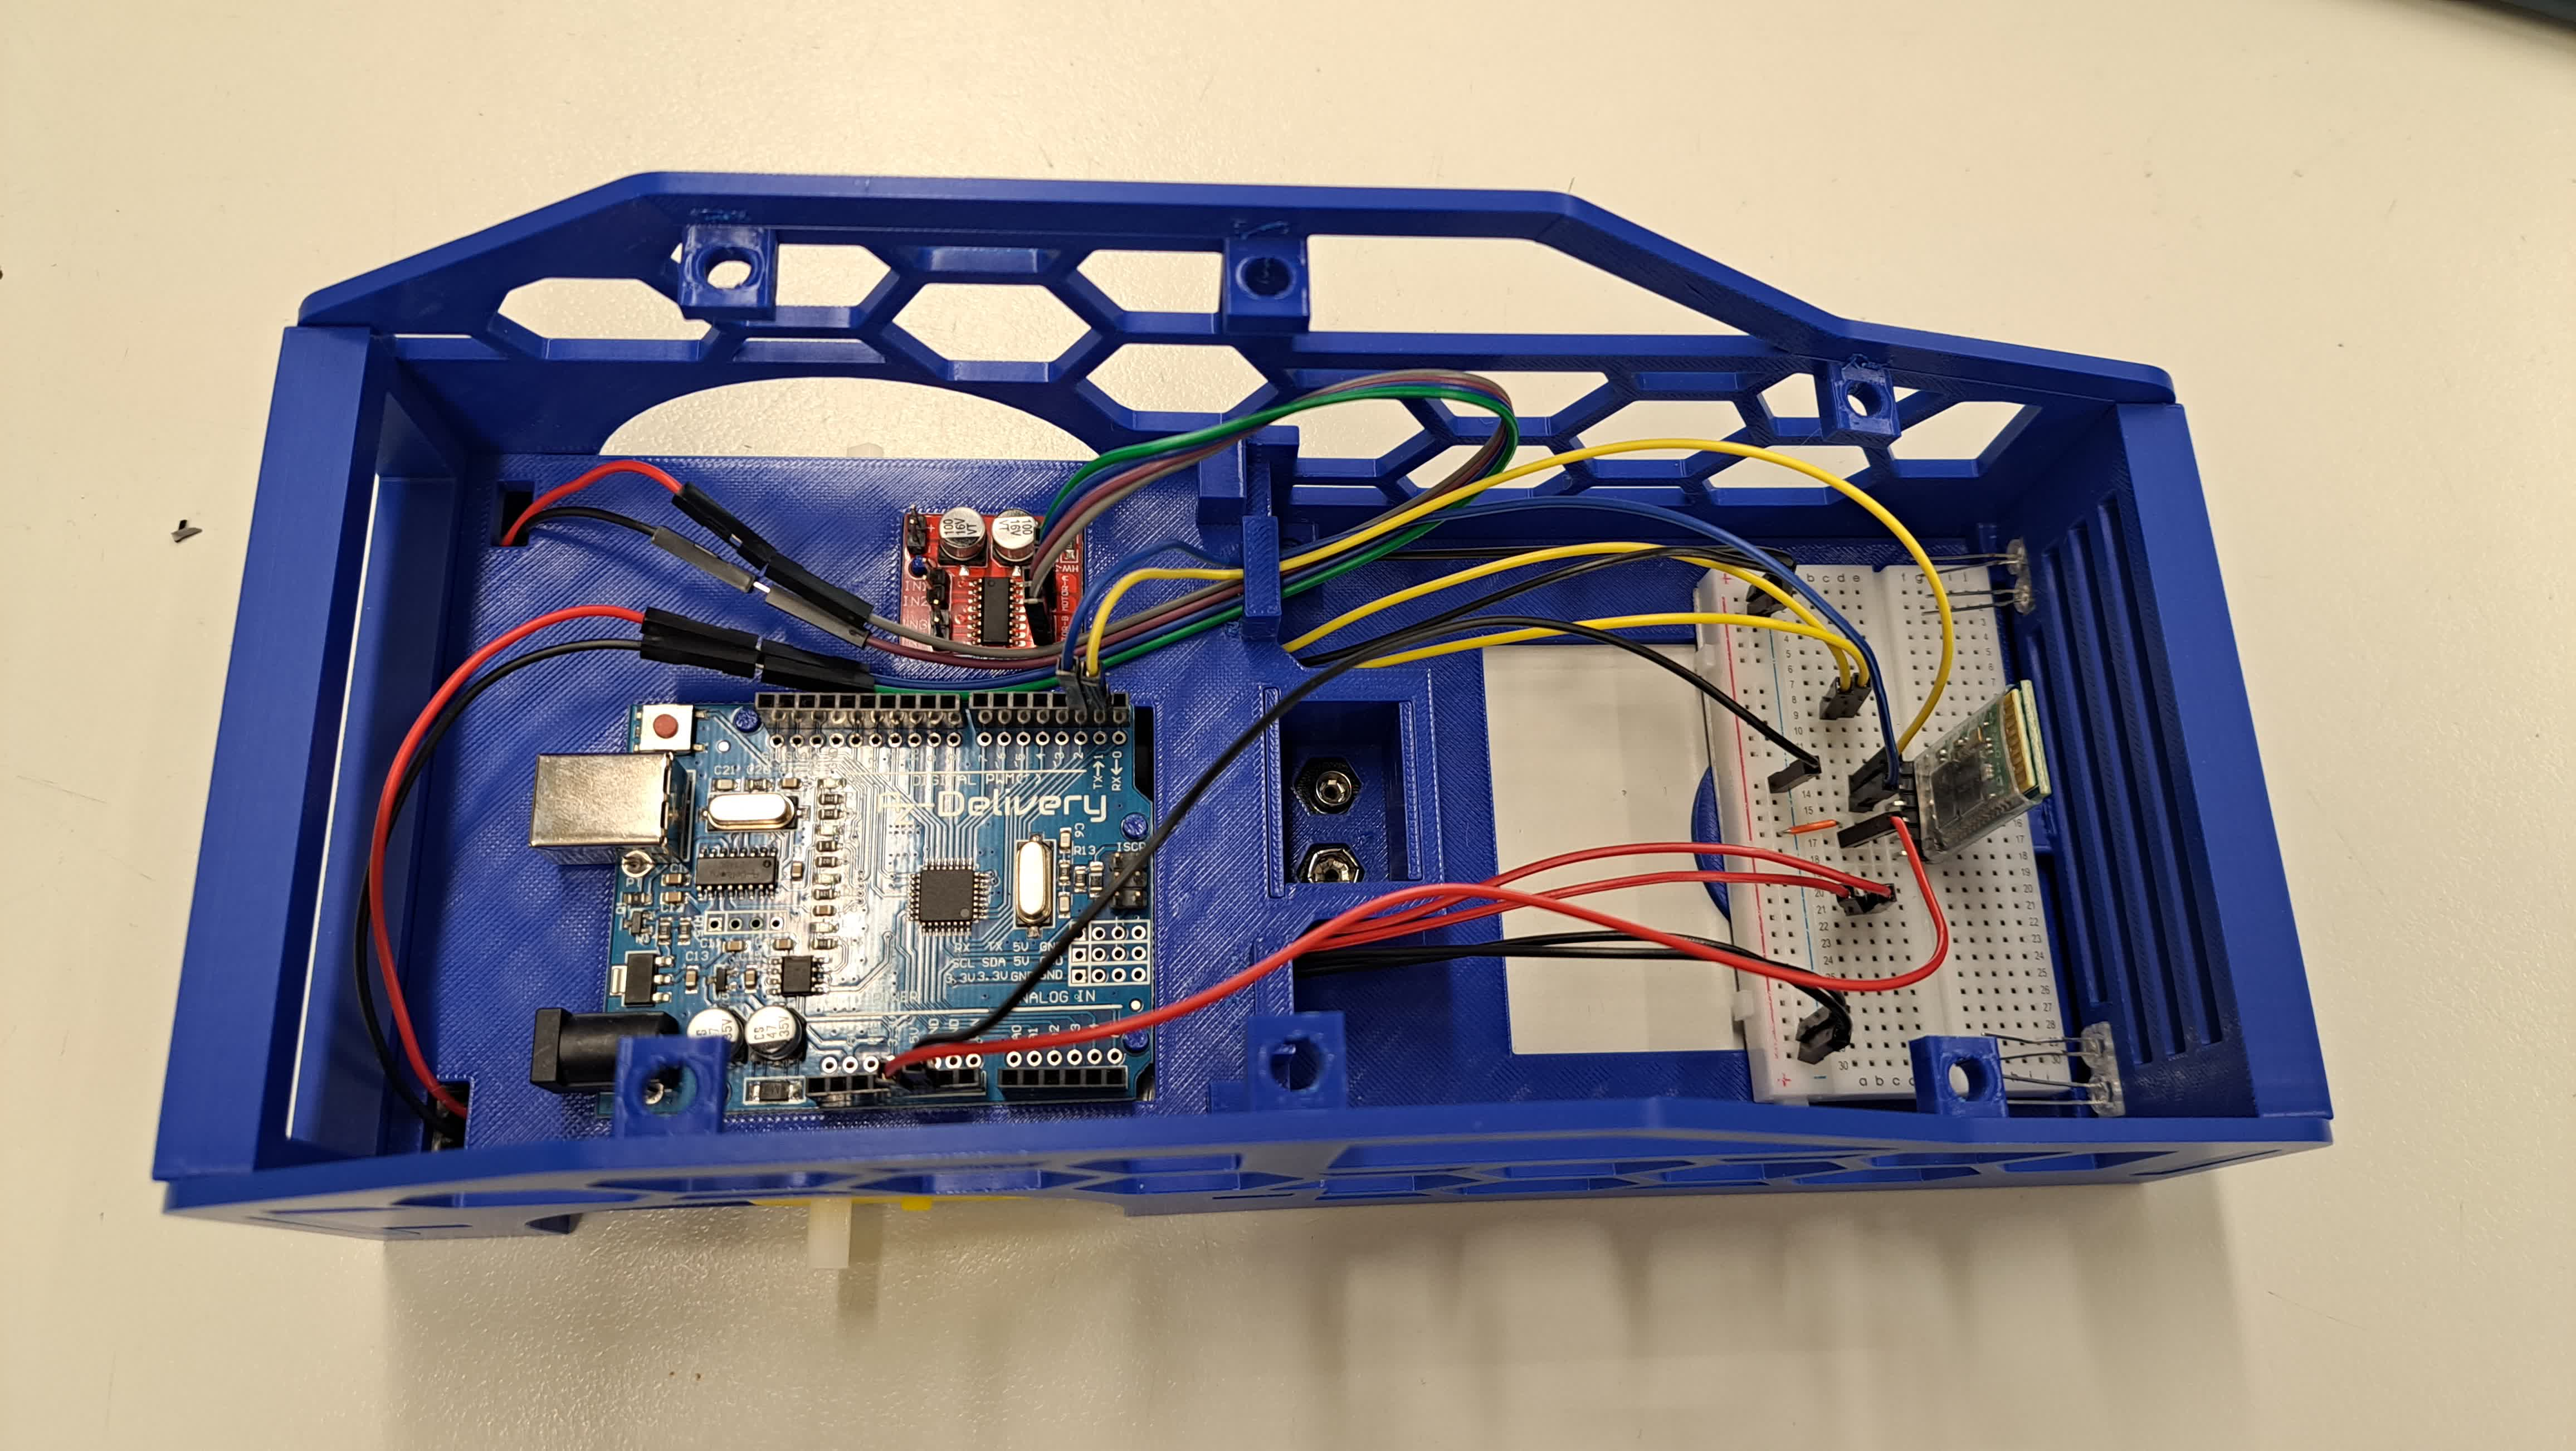
\includegraphics[width=0.9\imagewidth]{IMG_1014}
		\caption{Bodenplatte und Außenverkleidung mit Arduino}
		\label{fig:10}
	\end{subfigure}
	\caption{Bodenplatte und Außenverkleidung}
\end{figure}

Nun setzt ihr die Bodenplatte auf die Außenverkleidung und schiebt die Kabel von den Motoren durch die Löcher am Ende der Platte, wie in Bild \ref{fig:9} zusehen ist. Dann packt ihr Female-Male Kabel in die Enden der Kabel, die ihr durch die Löcher geführt habt und zu den Motoren führen. Die Female-Enden gehören jeweils paarweise an die H-Brücke, wobei der linke Motor an Motor-A soll. 

Anschließend könnt ihr die Bodenplatte mit dem Arduino zusammenbauen wie in Bild \ref{fig:10} zu sehen ist. Auf Bild \ref{fig:10} seht ihr auch, wie die Kabel der Rücklichter unter der Mittelplatte nach vorne geführt werden (rote, gelbe und schwarze Kabel) und die schwarzen Kabel alle in die Minusreihe des Steckbretts gesteckt werden und die gelben und roten Kabel, jeweils in eine Reihe gesteckt werden. 

Nun soll auch der Bluetooth Sender angeschlossen werden. Dazu steckt ihr den HC05 in das Steckbrett und verbindet die Kabel wie in Bild \ref{fig:10} zu sehen ist. Das rote Kabel wird an 5V des Arduinos, das schwarze Kabel an die Minusreihe des Steckbrettes und das gelbe Kabel an RX angeschlossen und beim Arduino an Pin 3. Das blaue TX Kabel wird an Pin 2 angeschlossen. Zum Schluss wird noch ein schwarzes Kabel an GND am Arduino angeschlossen und an die Minusreihe des Steckbrettes.

\begin{figure}[H]
	\centering
	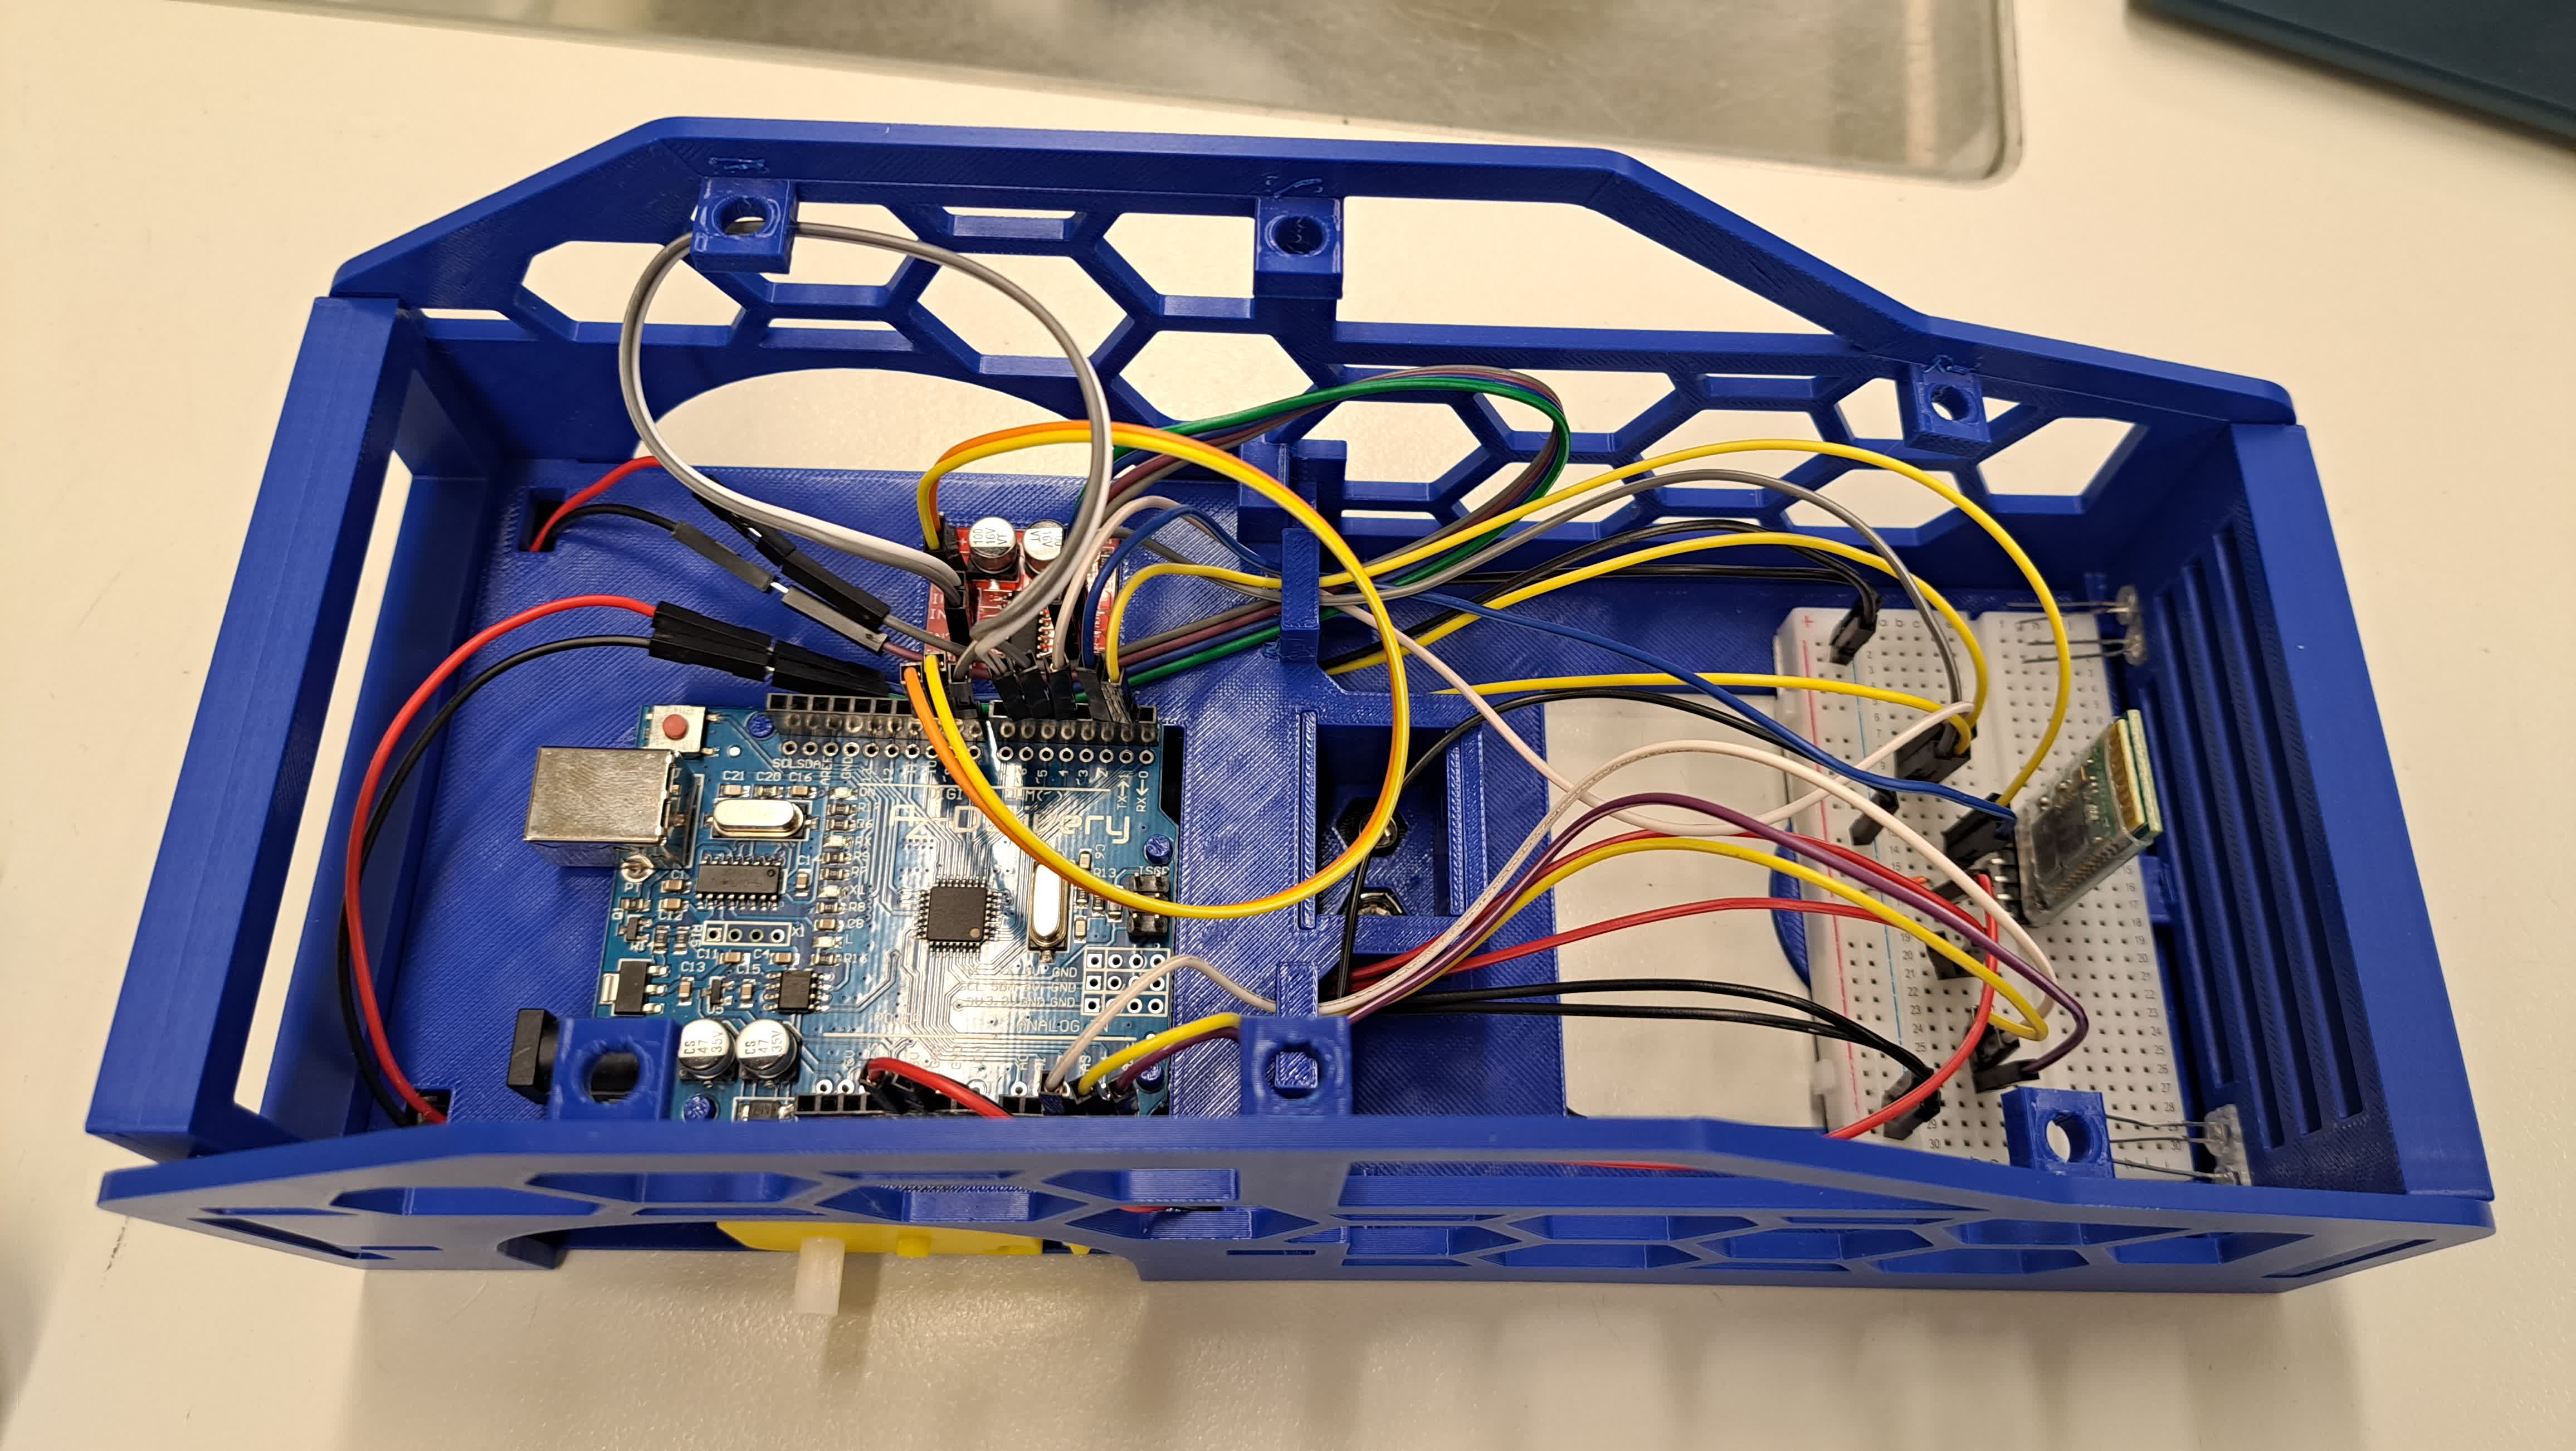
\includegraphics[width=\imagewidth]{IMG_1015}
	\caption{Weitere Verkabelung}
	\label{fig:11}
\end{figure}

Nun schließen wir die H-Brücke und die Lichter an den Arduino an. Dazu steckt ihr die Kabel der H-Brücke in die Pins 5, 6, 9 und 10. Die Kabel für die Lichter wie folgt: Pin 4 für die rechten Blinker, Pin 8 für die linken Blinker, Pin A2 für die Rücklichter, Pin A4 für das rechte Frontlicht und Pin A5 für das linke Frontlicht. Nun müsst ihr nur noch die passenden Kabel zusammen auf dem Steckbrett verbinden und ihr seid fertig mit der Verkabelung.

\begin{figure}[H]
	\centering
	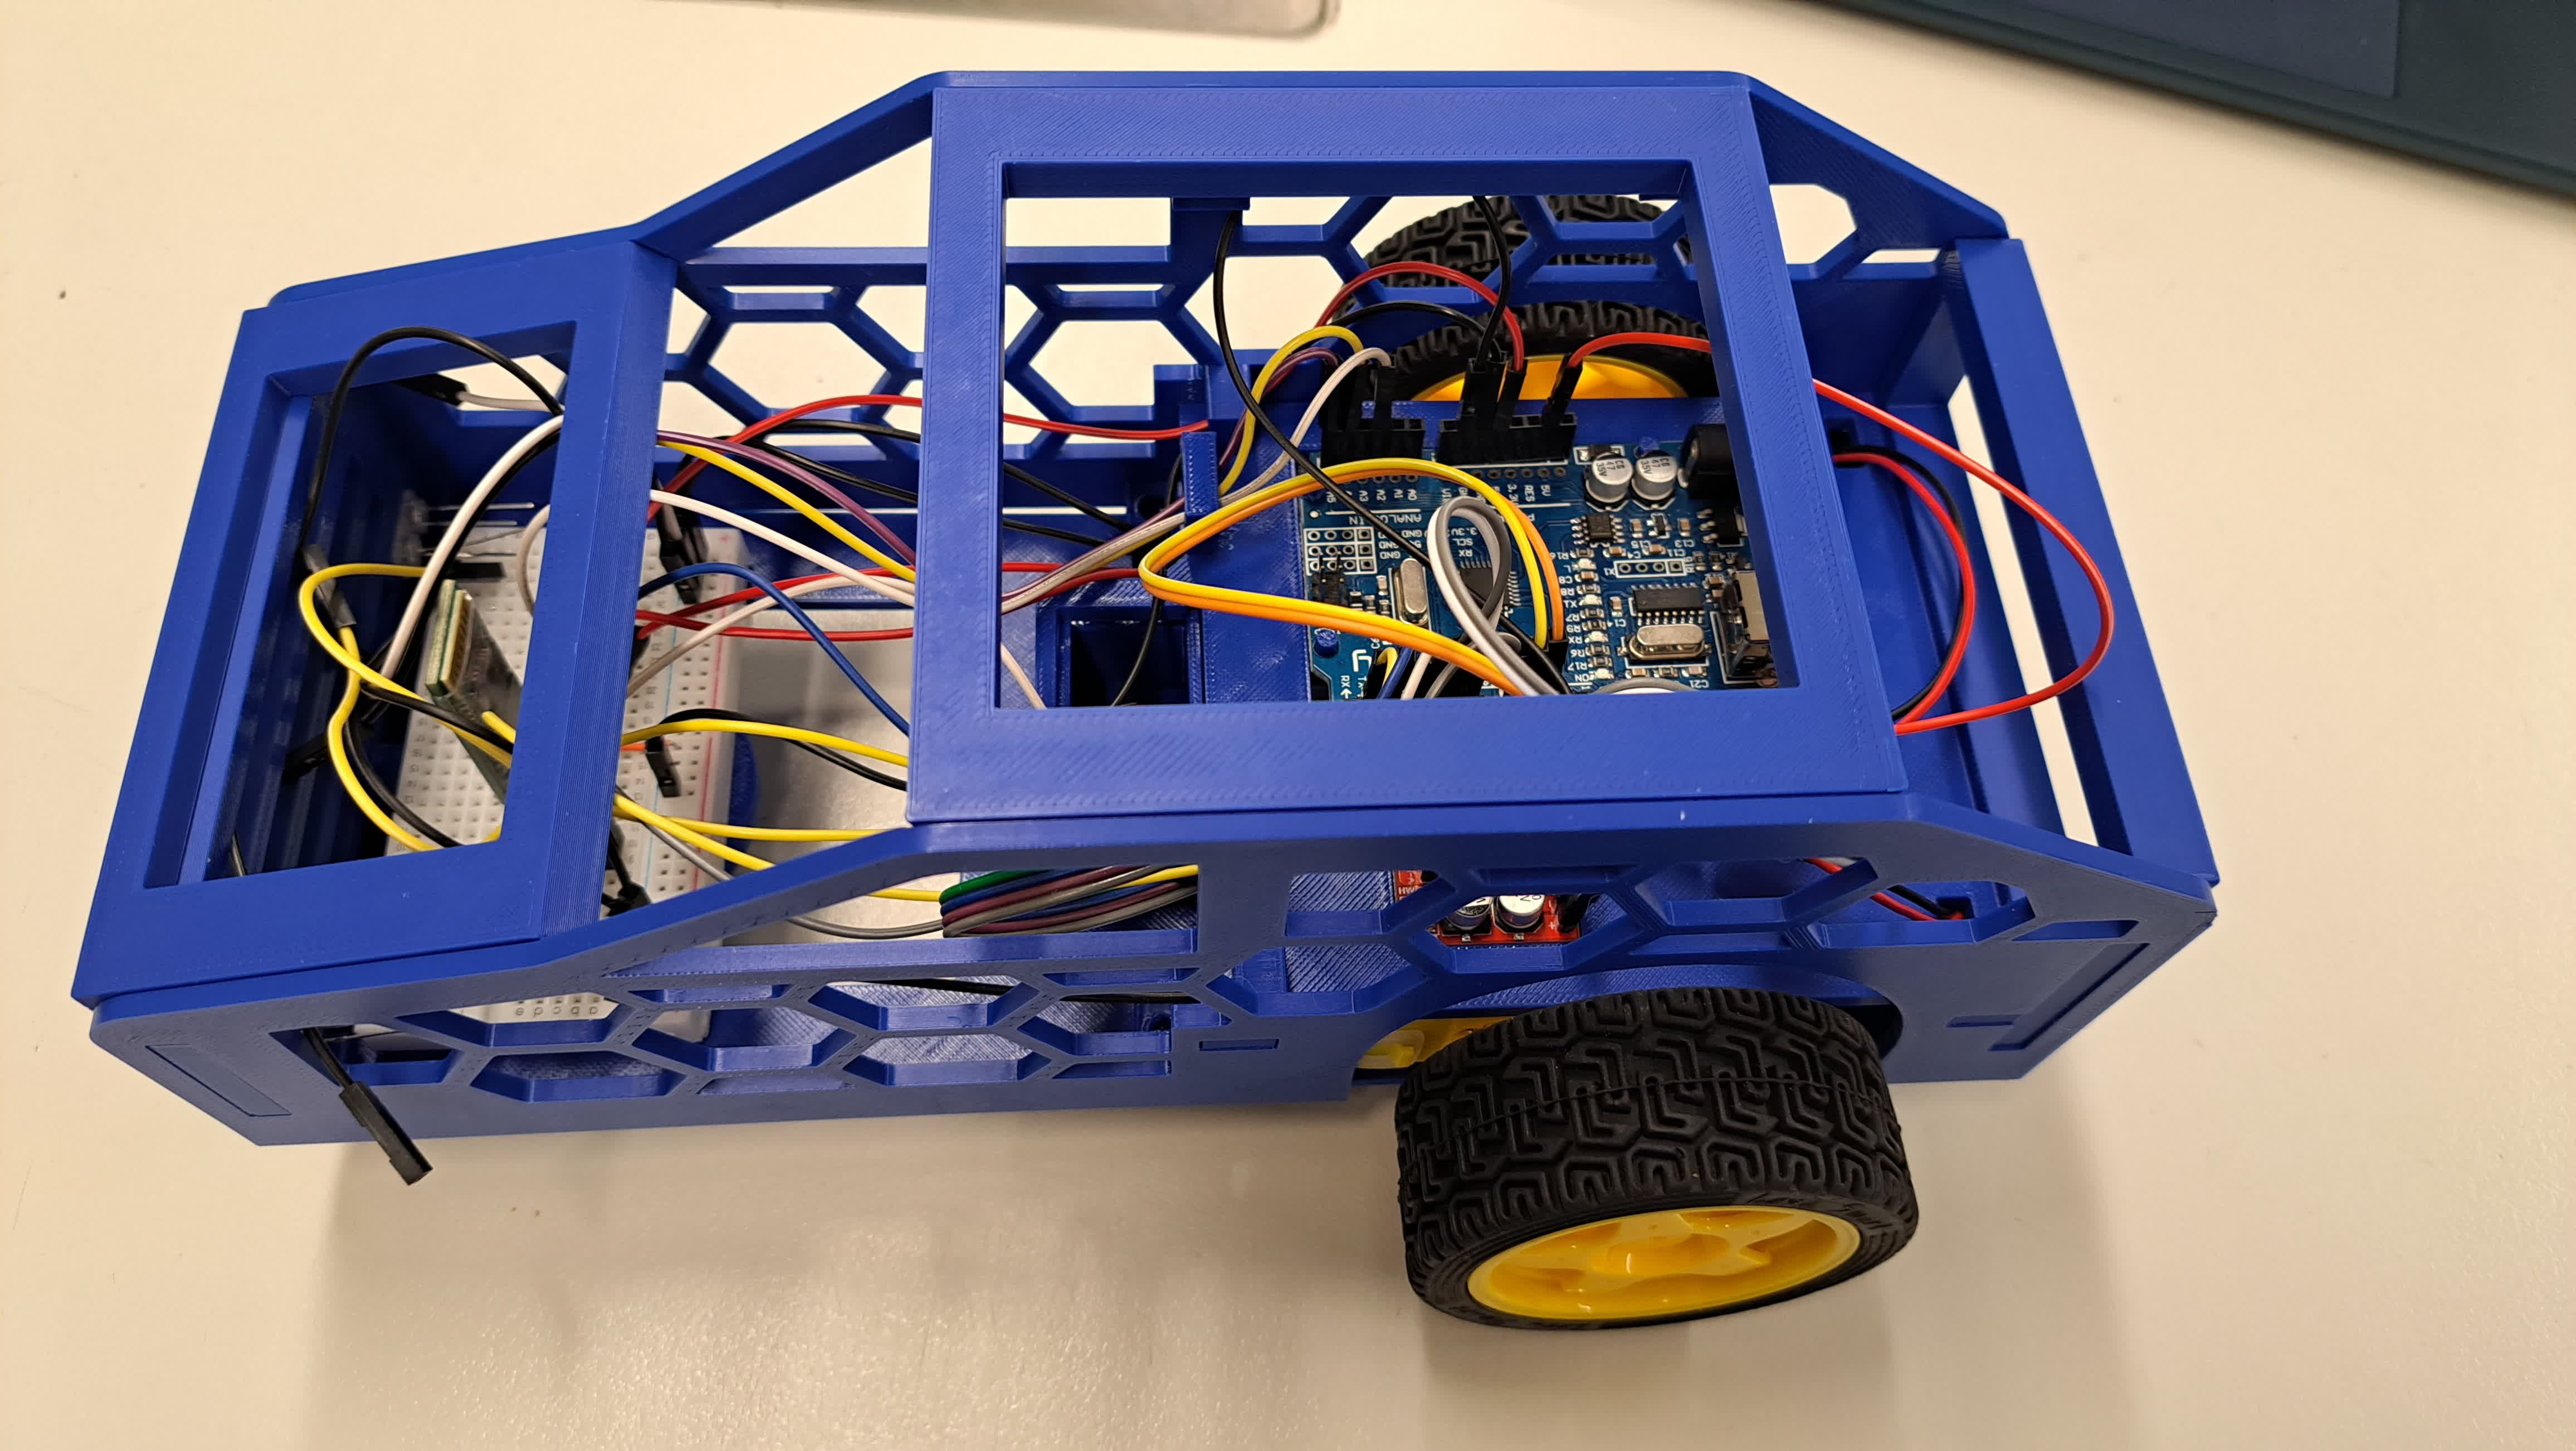
\includegraphics[width=\imagewidth]{IMG_1018}
	\caption{Fertig zusammengebaut}
	\label{fig:12}
\end{figure}

Zum Schluss kommen noch die obere Abdeckungen auf das Auto und ihr seid fertig mit dem Zusammenbau wie in Bild \ref{fig:12} zu sehen ist.

\end{document}
